\documentclass[UTF8,a4paper]{ctexart}
\usepackage[margin=1in]{geometry}
\usepackage{fancyhdr,hyperref,xcolor,amsmath,float,graphicx,cancel}
\usepackage{tikz}
\usetikzlibrary{positioning}
\usetikzlibrary{automata}
\usetikzlibrary{arrows.meta}
\newcommand\hl{\bgroup\markoverwith
  {\textcolor[rgb]{0.9, 0.99, 0.9}{\rule[-.5ex]{2pt}{2.5ex}}}\ULon}

\pagestyle{fancy}
\hypersetup{hidelinks}

\lhead{\bfseries \leftmark}
\chead{}
\rhead{SCUT}
\lfoot{\url{https://github.com/285571052}}
\cfoot{qhy}
\rfoot{\thepage}
\setlength{\headheight}{13pt}
\renewcommand{\headrulewidth}{0.4pt}
\renewcommand{\footrulewidth}{0.4pt}

\setlength{\parindent}{0pt}
\newcommand{\spaceline}{\vspace{\baselineskip}}

\author{ qhy }
\date{\today}
\title{编译原理}
% \includeonly{}
\begin{document}
\maketitle
\tableofcontents
\newpage
  \section{介绍}

  \textbf{预期收货}:
  \begin{itemize}
    \item 通过学习编译原理,写出更高效的代码
    \item 针对目标,自编写编译器

    对某个模型机的编译器进行设计
  \end{itemize}

  \textbf{编译器和解释器的区别?}\\
  编译器是转换器,解释器是执行系统。

  \spaceline

  程序编译的过程主要分为两大阶段:
  \begin{itemize}
    \item [1.] 查错
    \begin{itemize}
      \item 词法分析
      \item 语法分析
      \item 语义分析
    \end{itemize}

    \item [2.] 综合(翻译)
    \begin{itemize}
      \item [1.] 产生中间代码进一步优化
      \item [2.] 目标代码生成
    \end{itemize}
  \end{itemize}

  高级程序处理过程:初始源程序$\to$预处理$\to$源程序$\to$编译$\to$目标汇编$\to$机器代码

  注:生成机器代码的时候,并不是直接生成,而是先生成对应的汇编代码,再生成机器代码。

  编译过程:每个阶段的输出作为下一个阶段的输入(即数据从一种形式转换成另一种形式)。

  编译过程的每个阶段都包括两个相同的处理:表格管理和出错处理。

  表格管理是保存编译过程每个阶段的数据和结果,出错处理则是对编译过程遇到的语法,词法等错误进行处理。

    \subsection{词法分析}
    主要分为两大步骤,扫描和分解

    扫描为从左到右扫描

    分解为以介符对语句进行分割(注:双引号内的介符不可划分)

    最后结果使用一个二元组保存,格式为(种类,值)

    \subsection{语义分析}
    语义分析:不断构造语法树

    如:类型不对,数组越界等

    过程:单词符号串$\to$语法分析$\to$语法短语

    识别规则:描述程序结果的规则,通常由递归规则表示。

    输出:合法的语法树

    \subsection{语义分析}
    语义分析:包括静态语义和动态语义

    常见的错误包括类型不匹配,数组越界等

    输出:生成中间代码

    结果使用四元式表示,格式为:(运算符,运算对象1,运算对象2,结果)

    \subsection{代码优化}
    代码优化:对代码进行优化化简

    \subsection{目标代码生成}
    目标代码生成:与目标机器紧紧相关,先生成对应的汇编代码,再生成机器代码

    \subsection{表格管理与出错处理}
    表格管理与出错处理:每个阶段都执行这一操作

    \subsection{编译程序划分}
    编译程序划分:分析与综合(翻译)两个阶段

    按是否与目标机器相关:前端(无关)和后端(相关)

  \section{文法和语言}

  掌握自下而上和自上而下的分析方法。

  \spaceline
  \textbf{程序设计的定义:}语言是一个记号系统。

  \textbf{分析程序设计语言的两个阶段:}$\left \{\begin{array}{l} \text{每个程序的构成规律}\\\text{每个程序的含义}\end{array} \right .$

    \subsection{语法}
    \textbf{语法:}是一组规定,用它可以形成和产生一个合适的程序。

    描述工具:文法

    语法只可以判断结构是否合法。

    \subsection{语义}
    \textbf{语义:}$\left \{ \begin{array}{l}\text{静态语义}\\\text{动态语义} \end{array} \right.$

    \spaceline

    \textbf{静态语义:}一系列限定的规则,确定哪些合乎语法的程序是合适的。

    \textbf{动态语义:}运行或动态链接时进行的判断。

    描述工具:指称语义,操作语义

    作用:检查类型匹配,变量作用域等。

    \subsection{文法}
    \textbf{如何描述语句?}
    \begin{itemize}
      \item [1.] 生成方式(文法)\\
      语言中每个句子可以用严格定义的规则进行构造
      \item [2.] 识别方式(自动机)\\
      用一个过程,经有限次计算后会停止回答"是" ,若属于句子,要么回答"否",要么永远持续下去
    \end{itemize}

    \spaceline
    \textbf{语言:}可以是有穷的也可以是无穷的,我们要做的是,找出语言的有穷表示。

    \textbf{文法的作用:}
    \begin{itemize}
      \item [1.] 使用有穷的规则描述无穷的语言
      \item [2.] 严格定义句子的结构,是判断句子结构是否合法的依据
    \end{itemize}

    \textbf{方法:}\\
    \hl{::=}表示定义一条规则\\
    \hl{$\Rightarrow$}表示应用这条规则,完成句子的变换(即由...推导出...的意思)

      \subsubsection{符号和符号串}
      \textbf{字符表(符号集):}由字母、数字和若干专用字符组成的非空有限集合。

      \textbf{符号串:}字母表中的符号组成的任何有穷序列。

      比如:$a,aca$是$A:\{a,b,c\}$的符号串。

      符号串的长度:符号串含有符号的个数

      符号串的运用:
      \begin{itemize}
        \item 连接\\
        定义:$x = "ST", y = "aby"$\\
        则$xy = "STaby"$

        \item 方幂\\
        $a^n = \begin{array}{c}\underbrace{aa\cdots aa}\\ \text{n个a} \end{array}$

        \item 集合的乘积\\
        定义:$A = \{a,b\} , B = \{0 ,1\}$\\
        则$AB = \{a0 , a1 , b0 , b1\}$\\
        注:A,B是符号串的集合,并且AB的结果中A的符号串在前面\\

        \item 集合的方幂\\
        $A^2 = AA$
      \end{itemize}

      \subsubsection{闭包}
      \textbf{闭包:}$\Sigma$的闭包为$\Sigma$上所有元素组合的集合$\Sigma^*$。即
      \begin{equation}
        \Sigma^* = \Sigma^0 \bigcup \Sigma^1 \bigcup \Sigma^2 \cdots
      \end{equation}

      \textbf{正闭包}:闭包去掉空集元素。即
      \begin{equation}
        \Sigma^+ = \Sigma^* - \{\phi\}
      \end{equation}

      \subsubsection{文法}
      \textbf{产生式(规则):}一组有序对$(\alpha , \beta)$ 表示$\alpha \to \beta$ 或$\alpha ::= \beta$

      \textbf{文法的定义:}四元组$(V_N,V_T , P , S)$

      其中,$V_N$表示非终结符 , $V_T$表示终结符 , $P$表示产生式集合,$S$表示文档其实符号。

      注:
      \begin{itemize}
        \item $S$为文档的其实符号,从具体情况上看,它就是句子本身,只是还没有经过解析。
        \item $V_N \bigcup V_T = 字母表$
      \end{itemize}

      例子:

      文法$G = (V_N,V_T , P , S)$\\
      $V_N = \{S\}, P = \{S \to 0S1 , S\to 01\}, V_T = \{0,1\}$\\
      开始符号为 $S$

      \spaceline
      文法$G = (V_N,V_T , P , S)$\\
      $V_N = \{\text{标识符,字母,数字}\}$\\
      $ V_T = \{a,b,\cdots,z,0,1,\cdots , 9\}$\\
      $P = \left \{
      \begin{array}{l}
      <\text{标识符}> \to <\text{字母}>,\\
      <\text{标识符}> \to <\text{标识符}><\text{字母}>,\\
      <\text{标识符}> \to <\text{标识符}><\text{数字}>, \\
      <\text{字母}> \to a,\\
      \cdots ,\\
       z,<\text{字母}>\\
       <\text{数字}> \to 0,\\
       \cdots ,\\
        9,<\text{数字}>
      \end{array}\right \}$\\
      $S = <\text{\text{标识符}}>$

      \subsubsection{简化表示}
      简化表示:只使用产生式来表示文法,四元组的其他三元在产生式中表示。
      \begin{itemize}
        \item 第一条产生式的左部表示$S$
        \item 用大写字母或者尖括号包围表示非终结符集合
        \item 用小写字母表示终结字符集合
        \item 左部相同的产生式的多个,可以用\hl{$|$}(或) 来简化表示。\\
        比如:$A\to \alpha , A \to \beta$可以简记为$A \to \alpha | \beta$\\
        注意:$A \to \alpha | \beta$表示的是两条产生式而不是一条,其中$\alpha , \beta$为候选式。
      \end{itemize}

    \subsection{归纳与推导}
    \textbf{直接归纳与直接推导:}\\
    若$v\Rightarrow w$则称$v$直接推导$w$ 或 $w$ 直接归纳为 $v$

    \spaceline

    \textbf{归纳与推导:}使用了多条产生式,记为
    \begin{equation}
      \renewcommand{\arraystretch}{0.5}
      S \begin{array}{c} + \\ \Rightarrow \end{array} \alpha
    \end{equation}
    或
    \begin{equation}
      \renewcommand{\arraystretch}{0.5}
      S \begin{array}{c} * \\ \Rightarrow \end{array} \alpha
    \end{equation}

    注:如果使用了一条产生式,进行了多次$\Rightarrow$也为直接推导, 推导是使用了多条产生式。

    \subsection{句型、句子、语言}
    \textbf{句型与句子的定义:}\\
    对于文法$G[S]$,若$\renewcommand{\arraystretch}{0.5}S \begin{array}{c} * \\ \Rightarrow \end{array} x$ ,则称$x$为文法$G$的句型。\\
    若$x$仅由终结符组成,则称$x$为文法$G$的句子

    注:
    \begin{itemize}
      \item 句型可以表示多个句子,句子是句型的一个情况之一。句子也是一个句型。
      \item 起始符也为句型,即\\
      隐含条件:$S\to S$ , 所以$S$也是文法$G$的句型。
    \end{itemize}

    \spaceline
    \textbf{语言$L[G]$的定义:}语言$L[G]$是文法$G[S]$的所有句子的集合。

    注:
    \begin{itemize}
      \item $+,(,*,$等出现在句子中的成分,也是终结符。
      \item 可以通过产生式的具体表达,判断出某个操作的优先级。
    \end{itemize}

    \spaceline
    \textbf{文法的等价:}\\
    若$L[G_1] == L[G_2]$ ,则称文法$G_1$ 和 文法$G_2$ 等价。

    \spaceline
    \textbf{文法的种类:}
    \begin{itemize}
      \item 0型文法\\
      对任一产生式$\alpha \to \beta$ , 都有$\alpha \in (V_N\cup V_T)$ ,且至少含有一个终结符,$\beta \in (V_N\cup V_T)$\\
      即 产生式左侧只要不是句子,就是0型文法
      \item 1型文法(上下文相关文法)\\
      在0型文法条件下,对任一产生式$\alpha \to \beta$ ,都有$|\beta| \leq |\alpha|$ , 仅仅$S \to \epsilon $除外($|\alpha|$指的是句型的长度)\\
      即产生式左侧短语右侧,就是1型文法
      \item 2型文法(上下文无关文法)\\
      在1型文法条件下,对任一产生式$\alpha \to \beta$ ,都有$\alpha \in (V_N) , \beta \in (V_N\cup V_T)$\\
      即产生式左侧只有非终结符\\
      大部分程序设计语言是2型文法
      \item 3型文法(正规文法)\\
      在2型文法的条件下,,对任一产生式$\alpha \to \beta$,都有形如$A\to aB$或$A \to a$,其中$A,B\in V_N , a \in V_T$\\
      即产生式的右侧必须是以终结符开头\\
      一般用来定义一个单词
    \end{itemize}
    4种类型的文法约束依次为:左侧不能是句子,左侧长度小于右侧,左侧只有非终结符,右侧以终结符开头

  \section{上下文无关文法及其语法树}
  上下文无关文法:2型文法,有足够的能力描述现今程序设计语言的语法结构

  例子:算数表达式:
  $E\to i|E+E|E*E|(E)$\\
  $<\text{赋值语句}> \to i := E$\\
  $<\text{条件语句}> \to if <\text{条件}> then <\text{语句}>$\\
  $| if <\text{条件}> then <\text{语句}> else <\text{语句}>$

  \subsection{规范推导和规范句型}
  \textbf{最左/右 推导}:\\
  在推导任何一步$\alpha\to \beta$时,其中$\alpha,\beta$为句型,都是对$\alpha$中的最左/右的
  非终结符进行替换,则成为最左/右推导。

  {\color{blue}推导到底是多次直接推导,还是多条产生式?前者}

  \textbf{规范推导:}最右推导\\
  \textbf{规范规约:}最左规约

  \textbf{语法树:}推导的过程,可以展开成语法树,但是从语法树是看不出语法树的构造顺序的(即推导的过程)\\
  在语法树上,从左到右读取叶子节点,可以得到句型或句子。

  \textbf{语法树的定义:}满足下面几个条件的树,则称为文法G的语法树。
  \begin{itemize}
    \item 每个节点都有标记,是终结符或者非终结符中一个符号
    \item 根节点的标记是起始符(S)
    \item 若一个节点至少有一个除它自己之外的子孙,则这个节点的标记一定是非终结符
    \item 语法树得到的一定是文法G的产生式
  \end{itemize}

  \textbf{文法的二义性:}\\
  一个文法存在某个句子对应2个不同的语法树,则称文法有二义性。

  \subsection{句型的分析}
  \textbf{句型的分析:}识别给定串是否是某文法的句型。

  句型的分析主要有两种方法:
  \begin{itemize}
    \item 自上而下的分析法(推导)
    \item 自下而上的分析法(规约)
  \end{itemize}

  \textbf{自上而下的算法:}从开始符出发,反复使用文法中的产生式,
  寻找匹配的推导。(从跟节点开始不断构造语法树,找出与给定串匹配的语法树)\\
  这个算法的关键之处是\textbf{如何选择产生式?}

  \spaceline
  \textbf{自下而上的算法:}从给定串出发,归约到起始符(从叶子节点出发,向上构造语法树)\\
  这个算法的关键之处是\textbf{如何确定可归约串?}

  自上而下的话,感觉就是凭空想象,直到退出想要的结果,而自下而上的话,则是从句子本身出发,带有明确的方向性,更为简单。

  \spaceline
  要确定可归约串,首先要了解\textbf{短语,直接短语,句子}的概念。{\color{red}为什么?回头需要去看算法的原理}\\
  \textbf{短语:}若$\renewcommand{\arraystretch}{0.5}S\begin{array}{c} * \\ \Rightarrow \end{array} \alpha A\delta
  \begin{array}{c} * \\ \Rightarrow \end{array} \beta$,则称$\beta$是句型{\color{red}$\alpha \beta \delta$}相对于$A$的短语。
    (从语法树上来看,短语就是叶子 或者 叶子与其父(祖宗)节点 的组合对应的句型 )

  {\color{blue}到底是句型$\alpha A \delta$ 还是 句型$\alpha \beta \delta$?后者}

  直接短语:若$\renewcommand{\arraystretch}{0.5}S\begin{array}{c} * \\ \Rightarrow \end{array} \alpha A\delta
   {\color{red}\Rightarrow}  \beta$,则称$\beta$是句型{\color{red}$\alpha \beta \delta$}相对于$A$的直接短语。
   (从语法树上来看,每个叶子都是直接短语)

   \textbf{句柄:}一个句型的最左直接短语为句柄(从语法树上来看,最左的叶子就是句柄)\\
   \textbf{可归约串}:句柄即可归约串。

   那么自下而上的算法则是,每次选取语法树的句柄归约。

   {\color{red} 后面补上一个求直接短语,短语, 句柄以及归约的例子}

   \spaceline
   \textbf{多余规则:}
   \begin{itemize}
     \item 不可到达
     \item 不可终止
   \end{itemize}

   \section{词法分析}
   \textbf{单词描述的工具:}正规文法(3型文法)和正则式(正则表达式)


   \subsection{正规文法与正则式}
   \textbf{正规文法}也称三星文法$G=(V_N , V_T , S , P)$,其P中的一条规则都有以下形式:$A\to aB$或$A \to a$,其中$A,B\in V_N , a \in V_T^*$。\\
   即(一句话概括)文法的产生式的右侧以终结符开头。

   \spaceline
   \textbf{正则式:}也称正则表达式。

   既然有了正规文法,为什么还需要正则式?(作用)\\
   因为正则式可以直观地看出单词的构成

   \spaceline
   给定集合$\Sigma$
   \begin{itemize}
     \item $\epsilon$和$\Phi$\footnote{$\Phi = \{\epsilon\}$}都是某个集合$\Sigma$上的正规式。
     \item 集合内的任意元素都是集合$\Sigma$的正规式
     \item 正规式经过以下运算之后,还是集合$\Sigma$的正规式
     \begin{itemize}
       \item "$|$" 或
       \item "$.$" 连接
       \item "$*$" 闭包
       \item 优先级 $* > . > |$
     \end{itemize}
   \end{itemize}

   例子:令$\Sigma = \{a,b\}$ , $\Sigma$上的正规式和相应的正规集的例子如下:
  \begin{table}[H]
  \centering
  \begin{tabular}{c|c}
  \hline
  正规式          & 正规集                                            \\ \hline
  $a$          & $\{a\}$                                        \\
  $a|b$        & $\{a,b\}$                                      \\
  $ab$         & $\{ab\}$                                       \\
  $(a|b)(a|b)$ & $\{aa,ab,ba,bb\}$                              \\
  $a^*$        & $\{\epsilon , a, aa,\cdots\}$,即任意个a的串          \\
  $(a|b)^*$    & $\{\epsilon , a, b ,aa ,ab\cdots\}$,即所有a,b组成的串 \\ \hline
  \end{tabular}
  \end{table}

  \subsection{正规文法和正则式的等价性}
  \textbf{将正规式转换成正规文法:}\\
  选择一个非终结符$S$生成类似产生式的形式:$S\to r$ ,并将$S$定为$G$的识别符号。\\

  \textbf{例子}:将$r = a(a|d)^*$转换成相应的正规文法。{\color{red}书本上貌似写多了,以下为自己观点}
  \begin{itemize}
    \item
    $S\to a(a|d)^*$
    \item
    $S\to aA$\\
    $A \to (a|d)^*$
    \item
    $S \to aA$\\
    $A \to (a|d)A$  \\
    $A \to \epsilon$
    \item
    $S \to aA$\\
    $A \to aA$\\
    $A \to dA$\\
    $A \to \epsilon$
  \end{itemize}

  {\color{red}为什么最右推导,最左规约是合理的?有什么直观的理解?}

  \subsection{有穷自动机}
  \textbf{有穷自动机}:也称有限自动机,是一种识别装置,能准确识别正规集,即识别正规文法所定义的语言和正规式所表示的集合。\\
  有穷自动机本质上是一个状态转移图。

  \spaceline
  \subsubsection{确定的有穷自动机(DFA)}
  定义:一个确定的有穷自动机$M$是一个五元组
  \[M = (K , \Sigma , f , s , z)\]
  其中,
  \begin{itemize}
    \item [(1)] K是一个有穷集,它的每个元素称为一个状态
    \item [(2)] $\Sigma$是一个有穷字母表,它的每个元素称为一个输入符号,所以也称为$\Sigma$为输入符号表。
    \item [(3)] f是转换函数, 是$K\times \Sigma \to K$上的映像。
    \item [(4)] $S\in K$,是唯一的一个初态
    \item [(5)] $Z \subseteq  K$,是一个终态集,终态也称为可接受状态或结束状态。
  \end{itemize}
  确定性体现在:
  \begin{itemize}
    \item 初态是唯一的
    \item 每个状态对应的唯一的下一个状态
  \end{itemize}

  \textbf{DFA可以使用状态图或状态矩阵表示:}图\ref{fig1}和图\ref{fig2}分别表示状态图和状态矩阵。

  \begin{figure}[H]
    \centering
    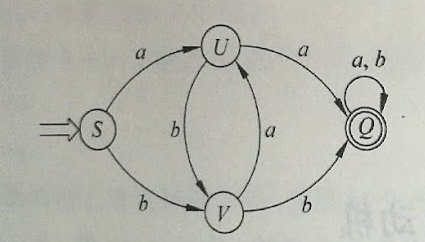
\includegraphics[scale = 0.3]{assets/CompilerConstructionPrinciples_5398e.png}
    \caption{状态转移图:初态结点冠以"$\rightarrow$"或标以"$-$",终态结点用双圈表示或标以"$+$"}
    \label{fig1}
  \end{figure}

  \begin{figure}[H]
    \centering
    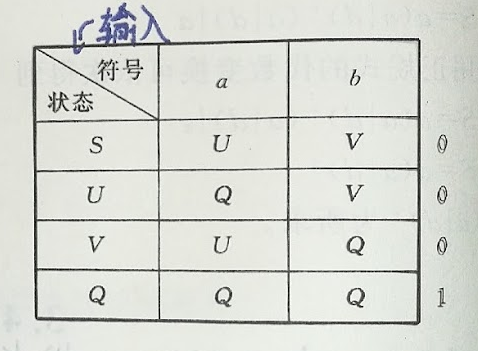
\includegraphics[scale = 0.3]{assets/CompilerConstructionPrinciples_c1ff8.png}
    \caption{状态转移矩阵:可以用$\rightarrow$标明初态;否则第一行即初态,相应终态行在表的右端标以1,非状态标以0}
    \label{fig2}
  \end{figure}

  \subsubsection{不确定的有穷自动机(NFA)}
  定义:一个不确定的有穷自动机$M$是一个五元组
  \[M = (K , \Sigma , f , s , z)\]
  其中,
  \begin{itemize}
    \item [(1)] K是一个有穷集,它的每个元素称为一个状态
    \item [(2)] $\Sigma$是一个有穷字母表,它的每个元素称为一个输入符号,所以也称为$\Sigma$为输入符号表。
    \item [(3)] f是转换函数, 是$K\times {\color{red}\Sigma^*}$到$K$的全体子集的映像,即$K\times {\color{red}\Sigma^*} \to 2^K$,其中$2^K$表示$K$的幂集
    \footnote{$K\times  Sigma^*$指的是两者的笛卡尔积,表示一个状态与每个输入的组合 ,
    然后这里取闭包$\Sigma^*$,表示每个状态与多个可能输入的组合(也可以分解成一个状态一个输入,这样写应该是为了简化,因为画图的时候,采取前者而不是逐个画)}
    \footnote{所谓幂集(Power Set), 就是原集合中所有的子集(包括全集和空集)构成的集族}
    {\color{blue}这一段是什么鬼?见脚注}
    \item [(4)] $S\subseteq K$,是一个非空初态集
    \item [(5)] $Z \subseteq  K$,是一个终态集
  \end{itemize}
  确定性体现在:
  \begin{itemize}
    \item 初态不唯一(有初态集)
    \item 每个状态对应的在同一个输入,有多个可能的状态转移。(即映射不唯一,一个状态映射到所有状态的某个子集)
  \end{itemize}

  \subsubsection{NFA转换为等价的DFA}
  \textbf{定理:}设$L$为一个由NFA接受的集合,则存在一个接受$L$的DFA。

  \spaceline
  \textbf{子集法:}将NFA转换成接受同样语言的DFA\\
  为一个NFA构造相应的DFA的基本想法是让DFA的每一个状态对应NFA的一组状态。(即把可能转移的多个不确定的状态的组合表示成一个状态来看)
  具体算法见\ref{fig-zijifa}{\color{blue}在进行子集法的时候,也会有无用状态去掉}

  \begin{itemize}
    \item $\epsilon$合并\\
    经过$\epsilon$弧得到的状态可以合并成一个状态
    \item 状态合并\\
    当前状态所能直接转移到的所有状态合并成一个状态
    \item 状态集合I的$\epsilon$闭包\\
    $\epsilon-closure(I)$状态集I中的任何状态S经过任一条$\epsilon$弧而能到达的状态
    \item 状态集合I的$a$弧转换\\
    $move(I,a)$,所有那些可从$I$中的某个状态经过一条a弧而达到的状态的全体。
  \end{itemize}

  \begin{figure}[H]
    \centering
    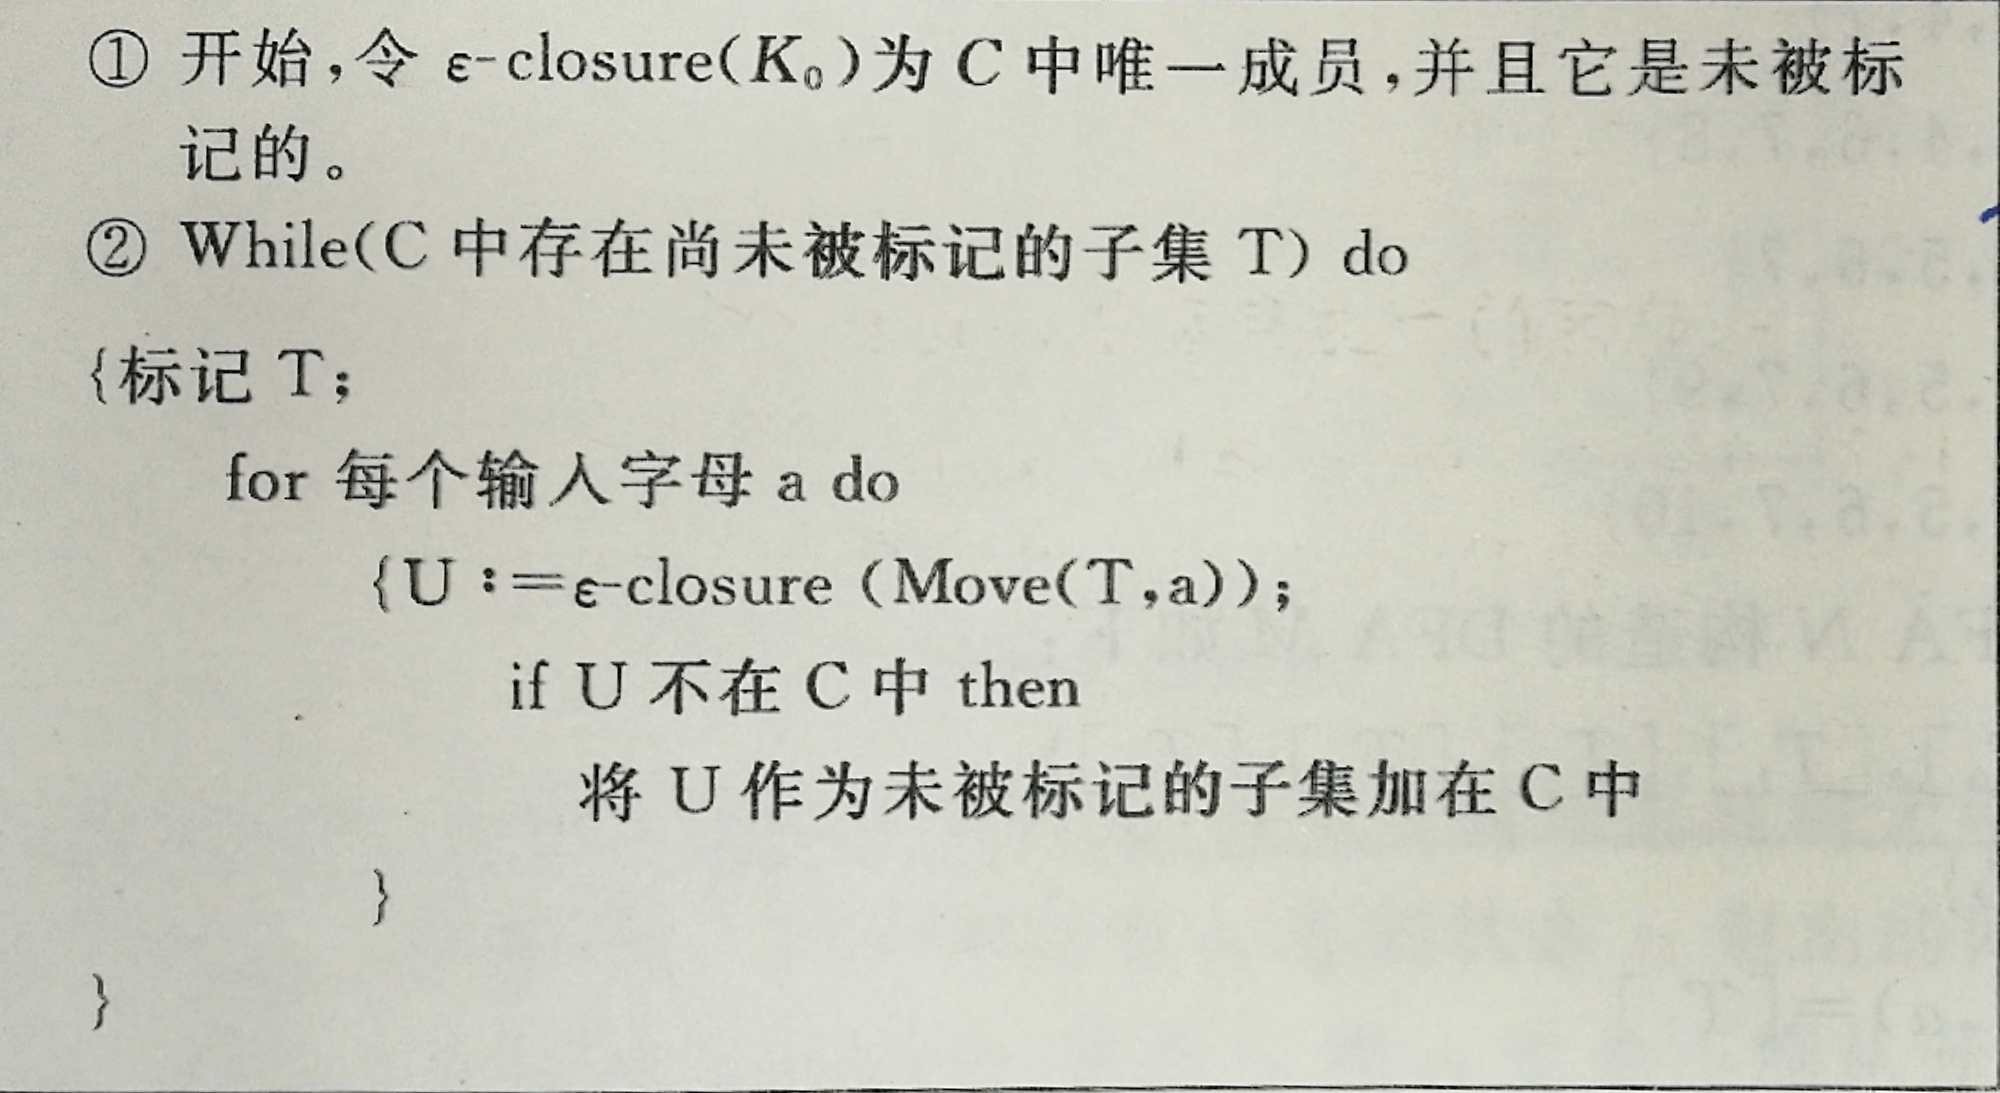
\includegraphics[scale = 0.1]{assets/CompilerConstructionPrinciples_763bd.png}
    \caption{子集构造算法}
    \label{fig-zijifa}
  \end{figure}

  \begin{itemize}
    \item C为DFA的状态集合,初始元素为起始状态的空闭包
    \item while所做的就是不断以C中的状态转移出新的状态加入C中,直到所有的装备都被使用过
    \item 所谓的转移,指的就是$\epsilon-closure(Move(T,a))$\\
    其中,$T$为C中的一个状态(它的值为NFA中某些状态的集合) , $a$表示经过的弧, 结果可以简记为$I_a$
    \item 终态的确定\\
    上面的算法确定的NFA对应到DFA有哪些状态,但是还未确定终态。\\
    DFA的\textbf{终态}就是DFA中和NFA中的终态有交集的状态。
  \end{itemize}

  \subsubsection{DFA的化简}
  一个DFA可以通过\textbf{消除无用状态}和\textbf{合并等价状态}来转换成一个等价的最小状态的DFA。\\
  也就是化简主要分两个部分。

  \spaceline
  所谓最简的DFA指的是它没有多余的状态,并且它的状态中没有两个是互相等价的。

  \spaceline
  \textbf{无用状态:}
  \begin{itemize}
    \item 从该自动机的开始状态出发,任何输入也不能到达的那个状态
    \item 从这个状态没有通路到达终态
  \end{itemize}
  {\color{blue}有什么算法能解决上面这个问题呢?从起点开始DFS,在能到达终点的前提下,所能访问到的所有的点都是有效的。其他都是无效的。\
  注:在进行子集法的时候,也会有无用状态去掉}

  \spaceline
  \textbf{等价状态:}
  \begin{itemize}
    \item [(1)] 一致性条件\\
    状态s和t的必须同时为可接受状态或不可接受状态。\footnote{可接受状态指的是终态,不可接受状态指的是非终态。}
    \item [(2)] 蔓延性\\
    对于所有输入符号,状态s和t必须转换到等价的状态里。
  \end{itemize}

  \spaceline
  那么如何找出等价的状态进而化简呢?\\
  \textbf{分割法:}把一个DFA(不含多余状态)的状态分成一些不相交的子集,使得任何不同的两个子集的状态都是可区别的,而
  同一子集中的任何两个状态都是等价的。

  \begin{itemize}
    \item 终态与非终态能初始划分出初始的两个不等价的子集。
    \item 对于每个集合,尝试所有的输入,如果集合内的两个状态不能转移到相同集合,那么这两个状态是不等价的,需要把这两个状态拆分到两个新的子集内。
    \item 尝试所有的输入可能,最终得到的集合内的元素就是相互等价的元素\\
    (因为尝试的所有的输入都是转移到相同的状态(可蔓延性) , 而一致性在初始的时候已经明确)。
  \end{itemize}

  \spaceline
  \textbf{例子:}把图\ref{example-zijifafengefa}表示的NFA确定化和最小化。
  \begin{figure}[H]
    \centering
    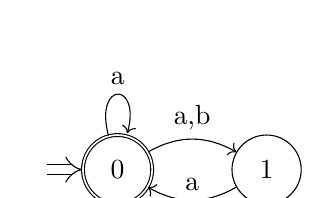
\begin{tikzpicture}
      [every initial by arrow/.style={double distance = 3,-Implies}]
    \node[state,initial,initial text=,double]  (A0)  {0};
    \node[state]  (A1)  [right=of A0] {1};

    \path [->] (A0) edge [bend left]  node [above] {a,b} (A1)
                  edge [loop above] node {a} (A0)
          (A1) edge [bend left] node [above] {a} (A0);
    \end{tikzpicture}
    \caption{例子:子集法、分割法例子}
    \label{example-zijifafengefa}
  \end{figure}

  \begin{itemize}
    \item 确定化,见表\ref{example-zijifa}
    \begin{table}[H]
      \centering
      \begin{tabular}{c|c|c}
        \hline
        set&input a&input b\\  \hline
        $A=\{0\}$ & $\{0,1\}(B)$ & $\{1\}(C)$\\
        $B=\{0,1\}$ & $\{0,1\}(B)$ & $\{1\}(C)$\\
        $C=\{1\}$ & $\{1\}(C)$ & $\Phi$\\
        \hline
      \end{tabular}
      \caption{例子:子集法 表}
      \label{example-zijifa}
    \end{table}

    对应状态图为:见图\ref{fig-example-zijifafengefa}
    \begin{figure}[H]
      \centering
      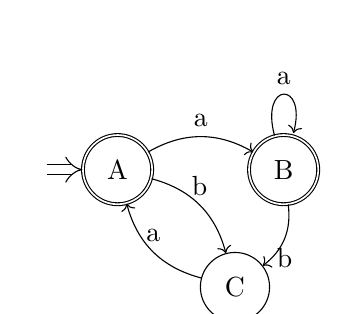
\begin{tikzpicture}[node distance=60,
        every initial by arrow/.style={double distance = 3,-Implies}]
      \node[state,initial,initial text=,double]  (A)  {A};
      \node[state,double]  (B)  [ right  of=A] {B};
      \node[state]  (C)  [below right  of=A] {C};

      \path [->] (A) edge [bend left]  node [above] {a} (B)
                 edge [bend left]  node [above] {b} (C)
                 (B) edge [loop above]  node [above] {a} (B)
                  edge [bend left]  node [below] {b} (C)
                (C) edge [bend left]  node [above] {a} (A);
      \end{tikzpicture}

      \caption{例子:子集法 图}
      \label{fig-example-zijifafengefa}
    \end{figure}
    \item 最小化,见表\ref{example-fengefa}
    \begin{table}[H]
      \centering
      \begin{tabular}{c|c}
        \hline
        input & sets\\  \hline
        init & $\{C\}$,$\{A,B\}$\\
        a & $\{C\}$,$\{A,B\}$ \\
        b & $\{C\}$,$\{A,B\}$\\
        \hline
      \end{tabular}
      \caption{例子:分割法 表}
      \label{example-fengefa}
    \end{table}

    因此$A,B$两个状态是等价的。
    对应的状态图为\ref{fig-example-fengefa}
    \begin{figure}[H]
      \centering
      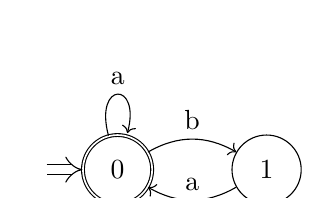
\begin{tikzpicture}
        [every initial by arrow/.style={double distance = 3,-Implies}]
      \node[state,initial,initial text=,double]  (A0)  {0};
      \node[state]  (A1)  [right=of A0] {1};

      \path [->] (A0) edge [bend left]  node [above] {b} (A1)
                    edge [loop above] node {a} (A0)
            (A1) edge [bend left] node [above] {a} (A0);
      \end{tikzpicture}
      \caption{例子:分割法 图}
      \label{fig-example-fengefa}
    \end{figure}

    另外,可以观察出,NFA的图\ref{example-zijifafengefa}和最小化后的DFA的图\ref{fig-example-fengefa}
    只是相差的一个$a$而已,实际上他们的确是等价的。\\
    因为  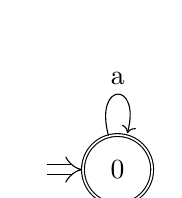
\begin{tikzpicture}
        [every initial by arrow/.style={double distance = 3,-Implies}]
      \node[state,initial,initial text=,double]  (A0)  {0};
      \path [->] (A0) edge [loop above] node {a} (A0);
      \end{tikzpicture}
    已经足够描述任意长度的a串,而无需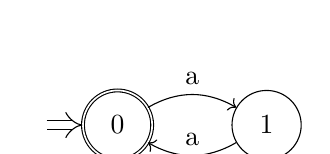
\begin{tikzpicture}
      [every initial by arrow/.style={double distance = 3,-Implies}]
    \node[state,initial,initial text=,double]  (A0)  {0};
    \node[state]  (A1)  [right=of A0] {1};

    \path [->] (A0) edge [bend left]  node [above] {a} (A1)
          (A1) edge [bend left] node [above] {a} (A0);
    \end{tikzpicture}
  \end{itemize}

  \subsubsection{正规式与有穷自动机的等价性}
  正规式和有穷自动机的等价性由以下两点说明:
  \begin{itemize}
    \item 对于字母表(输入表)$\Sigma$上的NFA M,可以构造一个$\Sigma$上的正规式r,使得$L(r) = L(M)$
    \item 对于$\Sigma$上的每个正规式r,可以构造一个$\Sigma$上的NFA M,使得$L(r) = L(M)$
  \end{itemize}

  \textbf{正规式$\to$NFA}:分两个步骤
  \begin{itemize}
    \item 建立x节点,使用$\epsilon$连接到初态,建立y节点,使用$\epsilon$弧连接终态
    \item 不断消去弧,直到只剩下x,y两个节点
  \end{itemize}
  消去规则:
  \begin{itemize}
    \item 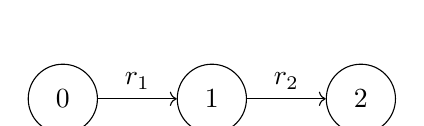
\begin{tikzpicture}
        [every initial by arrow/.style={double distance = 3,-Implies}]
      \node[state]  (A0)  {0};
      \node[state]  (A1)  [right=of A0] {1};
      \node[state]  (A2)  [right=of A1] {2};
      \path [->] (A0) edge  node [above] {$r_1$} (A1);
      \path [->] (A1) edge  node [above] {$r_2$} (A2);
      \end{tikzpicture} $\to$ 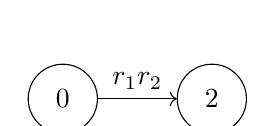
\begin{tikzpicture}
          [every initial by arrow/.style={double distance = 3,-Implies}]
        \node[state]  (A0)  {0};
        \node[state]  (A2) [right=of A0] {2};
        \path [->] (A0) edge  node [above] {$r_1r_2$} (A2);
        \end{tikzpicture}

    \item 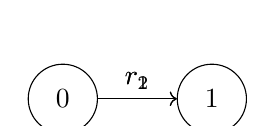
\begin{tikzpicture}
        [every initial by arrow/.style={double distance = 3,-Implies}]
      \node[state]  (A0)  {0};
      \node[state]  (A1) [right=of A0] {1};
      \path [->] (A0) edge  node [above] {$r_1$} (A1);
      \path [->] (A0) edge  node[above]  {$r_2$} (A1);
      \end{tikzpicture} $\to$ 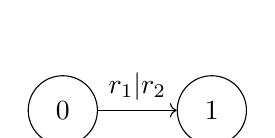
\begin{tikzpicture}
          [every initial by arrow/.style={double distance = 3,-Implies}]
        \node[state]  (A0)  {0};
        \node[state]  (A1) [right=of A0] {1};
        \path [->] (A0) edge  node[above]  {$r_1|r_2$} (A1);
        \end{tikzpicture}

    \item 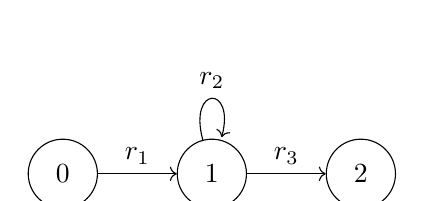
\begin{tikzpicture}
        [every initial by arrow/.style={double distance = 3,-Implies}]
      \node[state]  (A0)  {0};
      \node[state]  (A1) [right=of A0] {1};
      \node[state]  (A2) [right=of A1] {2};
      \path [->] (A0) edge  node[above]  {$r_1$} (A1);
      \path [->] (A1) edge  node [above] {$r_3$} (A2);
      \path [->] (A1) edge [loop above] node [above] {$r_2$} (A1);
      \end{tikzpicture} $\to$ 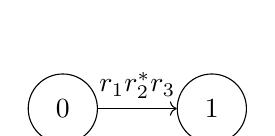
\begin{tikzpicture}
          [every initial by arrow/.style={double distance = 3,-Implies}]
        \node[state]  (A0)  {0};
        \node[state]  (A1) [right=of A0] {1};
        \path [->] (A0) edge  node[above]  {$r_1r_2^*r_3$} (A1);
        \end{tikzpicture}
  \end{itemize}

  \textbf{NFA$\to$ 正则式}:
  \begin{itemize}
    \item 环对应闭包\\
    注意,闭包是包括空的
    \item 连续输入对应与
    \item 分枝对应或
  \end{itemize}

  \subsubsection{正规文法和有穷自动机的等价性}
  主要有以下几点性质:
  \begin{itemize}
    \item 弧的输入(字母表)就是终结符
    \item 非终结符就是状态
    \item 新增一个状态Z作为终态
    \item 对于形如$A\to tB$的产生式,得到$f(A,t) = B$的转换函数。即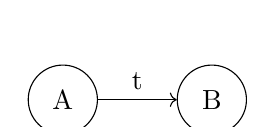
\begin{tikzpicture}
        [every initial by arrow/.style={double distance = 3,-Implies}]
      \node[state]  (A0)  {A};
      \node[state]  (A1) [right=of A0] {B};
      \path [->] (A0) edge  node[above]  {t} (A1);
      \end{tikzpicture}

    \item 对于形如$A\to t$的产生式,得到$f(A,t) = Z$的转换函数,即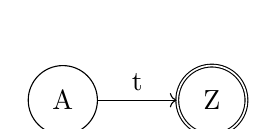
\begin{tikzpicture}
        [every initial by arrow/.style={double distance = 3,-Implies}]
      \node[state]  (A0)  {A};
      \node[state,double]  (A1) [right=of A0] {Z};
      \path [->] (A0) edge  node[above]  {t} (A1);
      \end{tikzpicture}
  \end{itemize}

  \textbf{正则式,正规文法,有穷自动机的关系?}\\
  正则式和正规文法是描述工具,有穷自动机是识别工具,三者可等价相互转换。

  \subsection{词法分析程序的构造}
  词法分析程序的构造主要分为4个步骤:
  \begin{itemize}
    \item 接口类型的确定\\
    语法分析程序可以有种利用方式:\\
    一是作为单独的子程序,其结果作为语法分析程序的输入。\\
    二是作为语法分析程序的一部分
    \item 确定单词的分类和Token串结构\\
    单词常见的类型有:关键字,标识符等\\
    token串一般为2元组(单词的种别,单词自身的值)  (需要自己对种类进行编号)

    \item 特殊问题
    \begin{itemize}
      \item 标识符和保留字的区分
      \item 空格、制表符及换行符的处理\\
      无用空格和制表符要删除\\
      字符串内的空格不能删\\
      换行符不能删,对于错误处理起作用
      \item 复合型Token的处理\\
      比如"!=" ,读取到"!"的时候,还必须读取下一个字符进行判断
      \item 括号,引号等成对符号的匹配问题\\
      这一个本应是语法分析的工作,但是可以词法分析程序中完成
    \end{itemize}

    \item 使用状态转换图构造语法分析程序
  \end{itemize}

  {\color{red}后面补上正规式,正规文法与有穷自动机相互转换的例子}

\textbf{综合例题:}
为正规文法$G[S]$\\
$S = \to aA|bQ$\\
$A \to aA|bB|b$\\
$B\to bD|aQ$\\
$Q\to aQ|bD|b$\\
$D\to bB|aA$\\
$E\to aB|bF$\\
$F\to bD|aE|b$\\
构造出相应的最小的DFA。
\begin{itemize}
 \item 正规文法$\to$NFA\\
       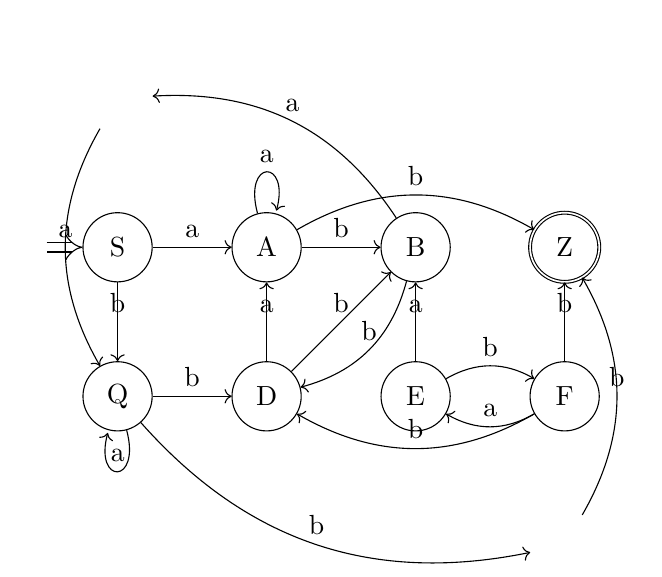
\begin{tikzpicture}
        [every initial by arrow/.style={double distance = 3,-Implies}]
        \node[state,initial,initial text=]  (S)  {S};
        \node[state]  (AA) [above=of S,draw=none] {};
        \node[state]  (A) [right=of S] {A};
        \node[state]  (B) [right=of A] {B};
        \node[state]  (E) [below =of B] {E};
        \node[state]  (D) [below =of A] {D};
        \node[state,double]  (Z) [right=of B] {Z};
        \node[state]  (F) [below=of Z] {F};
        \node[state]  (BB) [below=of F,draw=none] {};
        \node[state]  (Q) [below =of S] {Q};

        \path [->] (S) edge   node[above]  {a} (A)
        (S) edge   node[above]  {b} (Q)
        (A) edge [loop above]  node[above]  {a} (A)
        (A) edge   node[above]  {b} (B)
        (A) edge [bend left]  node[above]  {b} (Z)
        (B) edge [bend left]  node[above]  {b} (D)
        %(B) edge [out = 135, in = 135]  node[above]  {a} (Q)
        (B) edge [bend right]  node[above]  {a} (AA)
        (AA) edge [bend right]  node[above]  {a} (Q)

        (Q) edge [loop below]  node[above]  {a} (Q)
        (Q) edge   node[above]  {b} (D)
        %(Q) edge [out=-45 , in = -45]  node[above]  {b} (Z)
        (Q) edge [bend right]  node[above]  {b} (BB)
        (BB) edge [bend right]  node[above]  {b} (Z)

        (D) edge   node[above]  {b} (B)
        (D) edge   node[above]  {a} (A)
        (E) edge   node[above]  {a} (B)
        (E) edge [bend left]  node[above]  {b} (F)
        (F) edge [bend left]  node[above]  {b} (D)
        (F) edge [bend left]  node[above]  {a} (E)
        (F) edge   node[above]  {b} (Z);
       \end{tikzpicture}

\end{itemize}

\section{自顶向下的语法分析}
\subsection{确定的自顶向下的语法分析}

\textbf{确定分析的条件:}从文法的开始符号出发,如果能根据当前的输入符号(单词符号)\textbf{唯一地}确定选用那个产生式进行推导,则分析是确定的。

确定的分析有以下3种可能情况:
\begin{itemize}
 \item $S\to pA|bA$\\
       产生式的右部由终结符开头,同一个非终结符的不同的产生式由不同的终结符开头,我们可以直接地,唯一确定选用那个产生式
 \item $S\to Ap|Bq$\\
       产生式的右部以(非空)终结符开头,同一个非终结符的右部由不同的符号开头\\
       这种情况,我们无法确定选用哪个产生式,关键是 \textbf{判断产生式右部推出的开始符号集} , 若$A$和$B$的开始符号集不相交分析过程是确定的
 \item $A \to \epsilon$\\
       对于空产生式左部的非终结符,关键是 \textbf{判断该非终结符的后跟符号集},分析过程可能是确定的。
\end{itemize}

要进行确定的自顶向下分析,文法要满足 是 $LL(1)$文法

\textbf{开始符号集:}\\
设$G = (V_T , V_N , P , S)$是上下文无关文法。(产生式左侧只有非终结符)\\
$\renewcommand{\arraystretch}{0.5}
 FIRST(\alpha) = \{a | \alpha \begin{array}{c} * \\ \Rightarrow \end{array}  a \beta , a \in V_T , \alpha ,\beta\in V^*\}$\\
则称$\renewcommand{\arraystretch}{0.5}
 FIRST(\alpha)$为$\alpha$的\textbf{开始符号集} 或 \textbf{首符号集}。(可以包含空弧$\epsilon$)\\
{\color{blue} 也就是求产生式的第一个可能的终结符}

\spaceline
\textbf{后跟符号:}\\
设$G = (V_T , V_N , P , S)$是上下文无关文法,$A\in V_N , S$是开始符号\\
$\renewcommand{\arraystretch}{0.5}FOLLOW(A) = \{ a | S \begin{array}{c} * \\ \Rightarrow \end{array}
 \mu A\beta\text{且}a\in FIRST(\beta) ,\mu\in V^*_T , \beta\in V^+ \}$(特别的,\#表示输入串的结束符)\\
{\color{blue} 也就是求产生式第二个可能的终结符,但是只有在有空弧的情况才考虑即($\epsilon \in FIRST(A)$)}

\textbf{划重点:\# 不要忘了},初始状态:$\# \in FOLLOW(S)$

\spaceline
\textbf{选择符号集:}\\
一个产生式的选择符号集合SELECT 。给定上下文无关文法的产生式\\
$A\to \alpha , A\in V_N , \alpha \in V^*$\\
若$\renewcommand{\arraystretch}{0.5} \alpha \begin{array}{c} * \\ \cancel{\Rightarrow} \end{array} \epsilon $,\\
则$SELECT(A \to \alpha) = FIRST(\alpha)$\\
若$\renewcommand{\arraystretch}{0.5} \alpha \begin{array}{c} * \\ \Rightarrow \end{array} \epsilon $,\\
则$SELECT(A \to \alpha) = (FIRST(A) - \{\epsilon\})\cup FOLLOW(A)$\\
{\color{blue} 也就是可选的非终结符,在没空弧的情况就是$FIRST$ , 在有空弧的情况就还要考虑$FOLLOW$(同时去掉空弧)}

\spaceline
\textbf{LL(1)文法的充要条件}
\begin{itemize}
 \item 上下文无关文法
 \item 对于每个非终结符$A$的两个产生式$A \to \alpha ,A \to \beta$,满足
       \[SELECT(A\to a) \land SELECT(A \to \beta) = \phi\]
       其中,$\alpha , \beta$不同时能$\renewcommand{\arraystretch}{0.5} \begin{array}{c} * \\ \Rightarrow \end{array} \epsilon$\\
       {\color{blue}也就是同一个非终结符的产生式的第一个可能终结符不能相同}
\end{itemize}

\spaceline
\textbf{LL(1)文法的判别:}
\textbf{一个上下文无关文法是LL(1)文法的}充要条件$\to$SELECT集$\to$FIRST+FOLLOW$\to$$\epsilon$

 \textbf{1的含义:}1表明只需要向前看一个符号便可以决定选哪个产生式进行推导,类似的$LL(k)$文法需要向前看$k$个符号才可以确定选用哪个产生式

 \begin{itemize}
  \item 求能推导出$\epsilon$的非终结符
\begin{itemize}
  \item 标记每个非终极符的状态
  \item 使用直接推导能推导出空的,标记是
  \item 循环推导,直到标记表不再发生变换\\
        有些不确定能推导出空的非终结符后来确定可以的时候,它所在的产生式也可能推导出空,因此循环处理
\end{itemize}
  \item 求FIRST
        $a \to X_1 X_2 \cdots X_n$
        \begin{itemize}
         \item $X_1$不为空,$FIRST(a)=FIRST(X_1)$
         \item 对于前j个可达空,$FIRST(a) = FIRST(A) + FIRST(X_J) - \{\epsilon\}$
         \item 循环,直到FIRST不变
        \end{itemize}
  \item 求FOLLOW\\
        $A = aBC$
        \begin{itemize}
         \item C不能达到空,FOLLOW(B) = FOLLOW(C)
         \item 可以达空,FOLLOW(B) = FOLLOW(A) + FIRST(C)
         \item 循环直到FOLOW不再增加
         \item 初始 FOLLOW(S) = {$\#$}
        \end{itemize}
  \item 求SELECT\\
        根据定义进行即可
 \end{itemize}

 {\color{red}后面补上一个例子}

 \subsubsection{非LL(1)文法转LL(1)文法}
 不是LL(1)文法:
 \begin{itemize}
  \item 消除左递归
  \item 提取左公因子
 \end{itemize}

 \textbf{提取左公因子}:

 对于含有$A \to ab | ac$的文法,显然不是$LL(1)$文法

 我们可以提取左公因子转换成$LL(1)$文法:
$A\to aB , B\to b|c$

\spaceline
 \textbf{直接左递归:}$A \to Ab$,含有左递归的产生式,称为直接左递归

 \textbf{间接左递归:}$A\to Ba  , B \to Ab$,即$A\Rightarrow^+ A$,称为间接左递归

 \spaceline
 以直接左递归为例子:$A \to Aa, A \to b$

 有:
$Select(A\to Aa) \supseteq First(Aa) \supseteq First(b)$

$Select(A\to b)\supseteq First(b)$
 因此,含有左递归的文法都不是$LL(1)$文法

 \textbf{消除直接左递归}:

$S\to Sa|b$

 改写成

$S\to bS' , S' \to aS' | \epsilon$

 \textbf{消除间接左递归}:通过代入等方法把间接左递归变成直接左递归,对于间接左递归下,还嵌套有直接左递归,那么先消除直接左递归,再代入

 \subsection{不确定的自顶向下分析}
 对于非$LL(1)$文法,就不能确定选择哪个产生式规则,对于待选的产生式,采用回溯搜索,逐条试探的方式进行

 其实就是回溯算法啦

 \textbf{含有空弧的情况有什么特殊处理的地方吗?}

 \subsection{确定的自顶向下算法-实现}
 \begin{itemize}
  \item 递归子程序算法
  \item 预测分析法
 \end{itemize}

 \subsubsection{递归子程序法}
 \textbf{实现思想}:对文法中的每个非终结符编写一个递归过程,识别由该终结符推出的串。当非终结符含有多条产生式时,按当前输入属于哪条产生式的SELECT集可唯一确定(LL(1)文法)哪个产生式进行匹配。

 \begin{itemize}
  \item 当识别到终结符时与输入符号匹配并读取下一输入符。
  \item 当识别到非终结符时,则调用该终结符相应的过程
 \end{itemize}

 特点:
 \begin{itemize}
  \item 优点:简单直观,易于构造
  \item 缺点
        \begin{itemize}
         \item 对文法要求高,必须满足$LL(1)$文法
         \item 递归调用多
        \end{itemize}
  \item 实用性:许多高级语言,如Pascal、c 等编译系统常常采用此方法
 \end{itemize}

 \subsubsection{预测分析法}
 一个预测分析器由3个部分组成:
 \begin{itemize}
  \item 预测分析程序\\
        控制分析过程的进行
  \item 分析栈\\
        存放从文法开始符号出发的自顶向下的推导过程中等待匹配的文法符号。\\
        开始时放入 \textbf{\#} 和文法开始符号\\
        结束时栈应该是空的。
  \item 预测分析表\\
        是一张二维表,元素$M[A,a]$的内容是当前非终结符面临输入符号a时应该选取的产生式\\
        当无产生式时,元素内容为转向出错处理
 \end{itemize}

 \textbf{构造预测分析表}:
 \begin{itemize}
  \item 把文法转变为$LL(1)$文法
  \item 求出每条产生式的$SELECT$集
  \item 依照$SELECT$集把产生式填入分析表
  \item 用a表示终结符或 \textbf{\#} ,若$a\in SELECT(A\to b)$,则把$A\to b$放入$M[A,a]$中,把所有无定义的$M[A,a]$标上出错标记
 \end{itemize}

\begin{figure}[H]
  \centering
  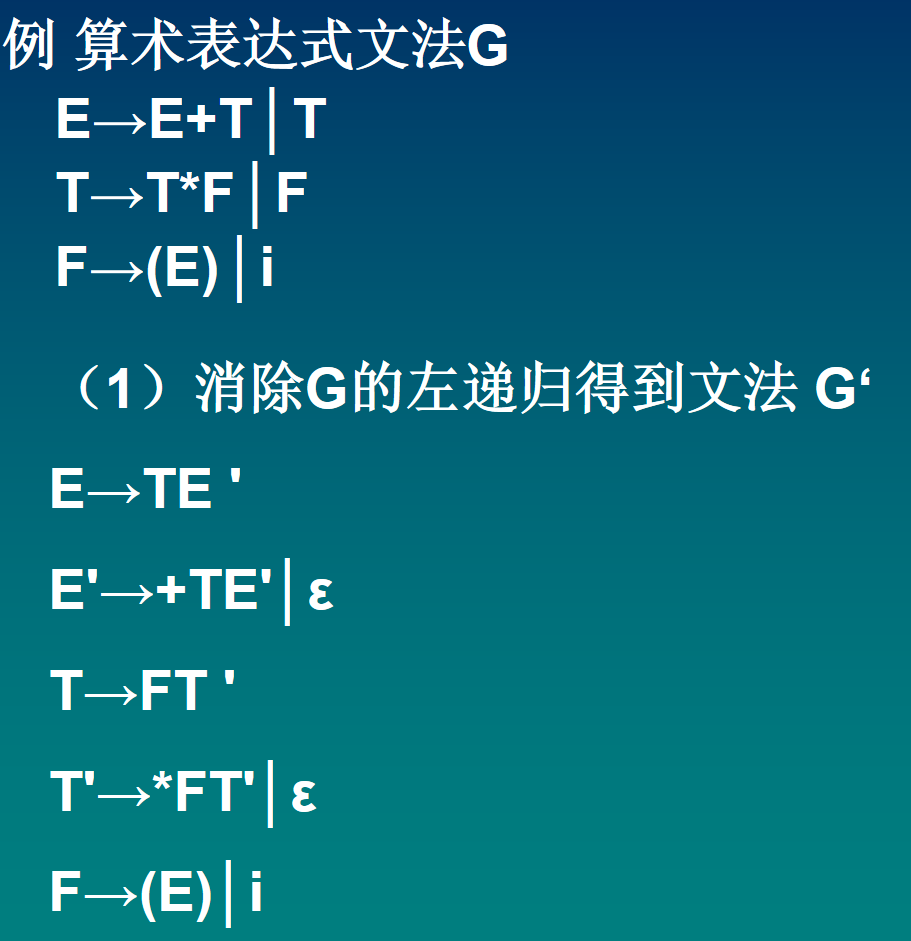
\includegraphics[scale = 0.3]{assets/CompilerConstructionPrinciples_7723b.png}
\end{figure}

 \begin{figure}[H]
  \centering
  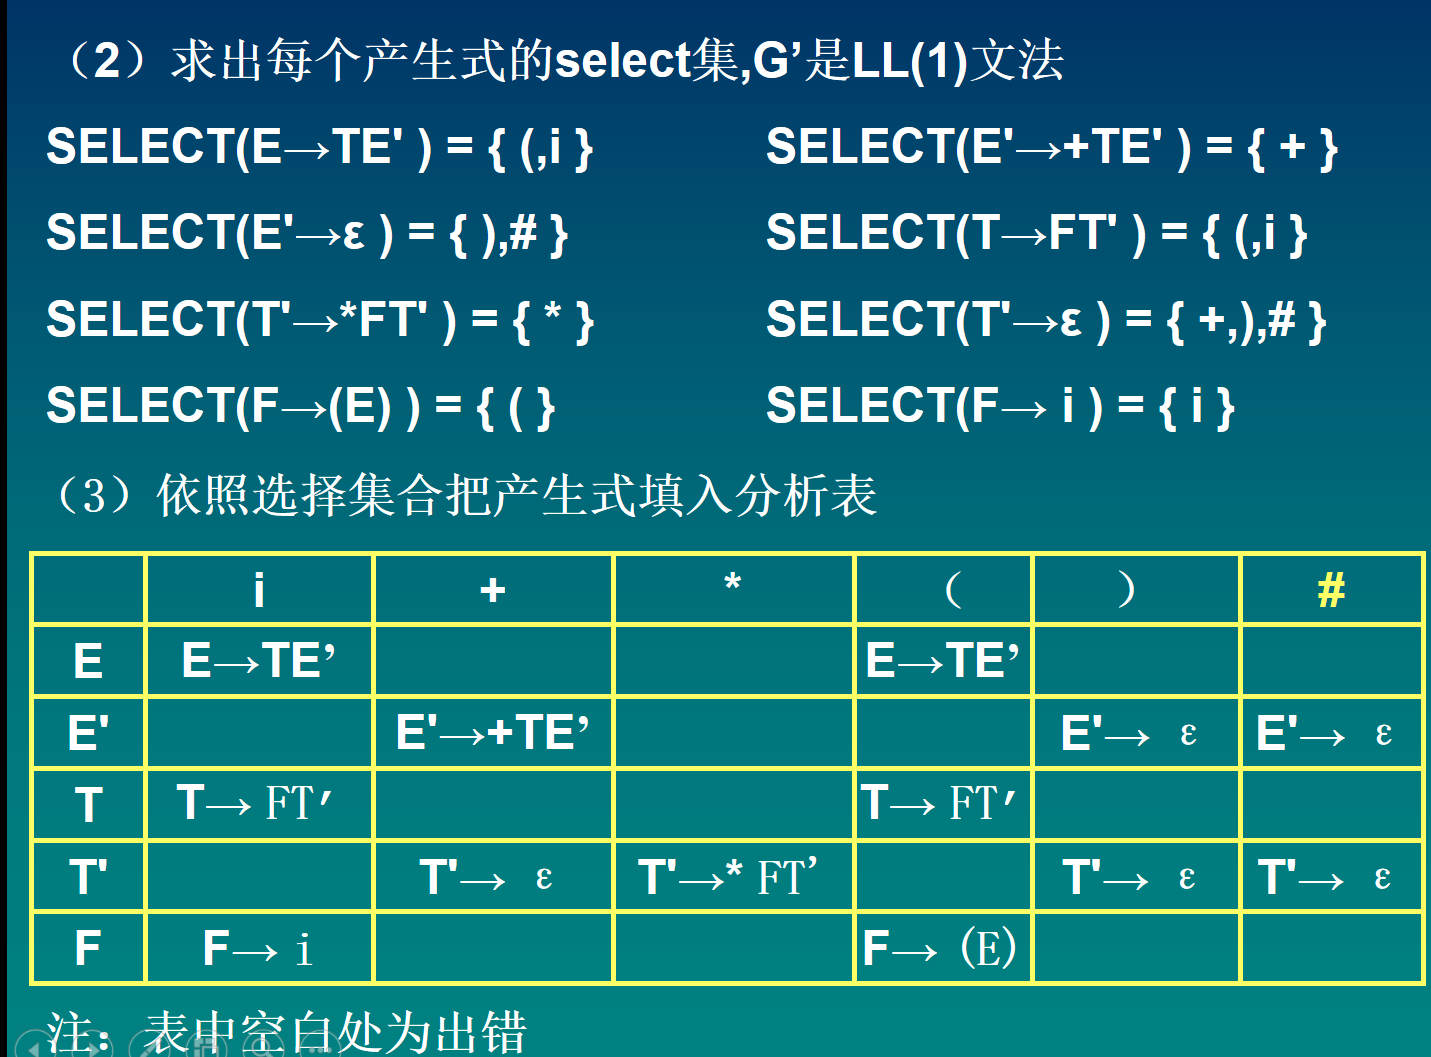
\includegraphics[scale = 0.3]{assets/CompilerConstructionPrinciples_7a51c.png}
 \end{figure}

 \begin{figure}[H]
   \centering
   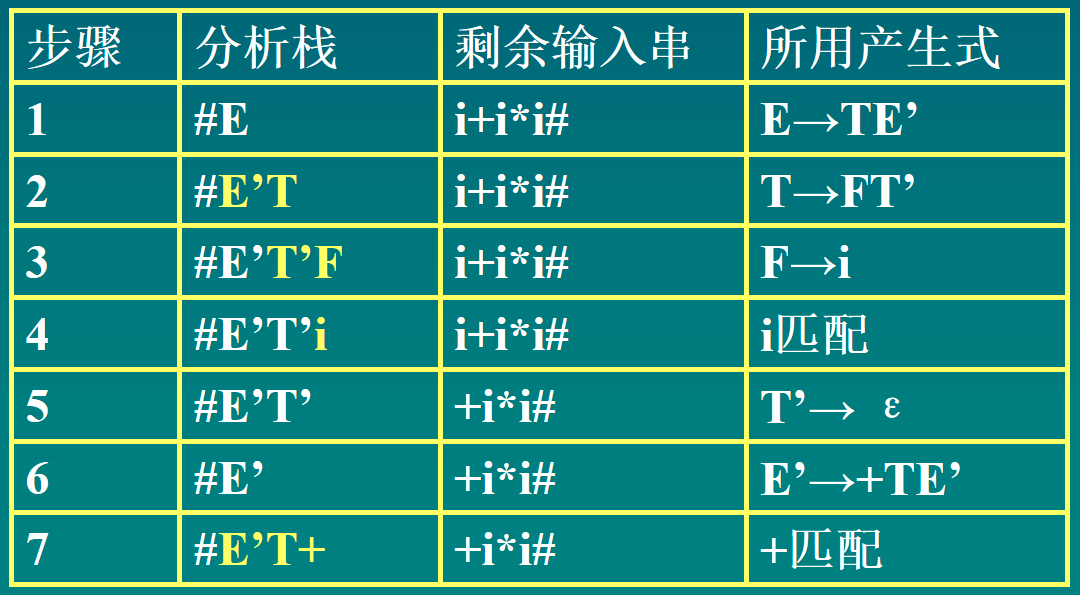
\includegraphics[scale = 0.3]{assets/CompilerConstructionPrinciples_0adb6.png}
   \caption{描述'i+i*i'的分析过程}
 \end{figure}
 \begin{figure}[H]
   \centering
   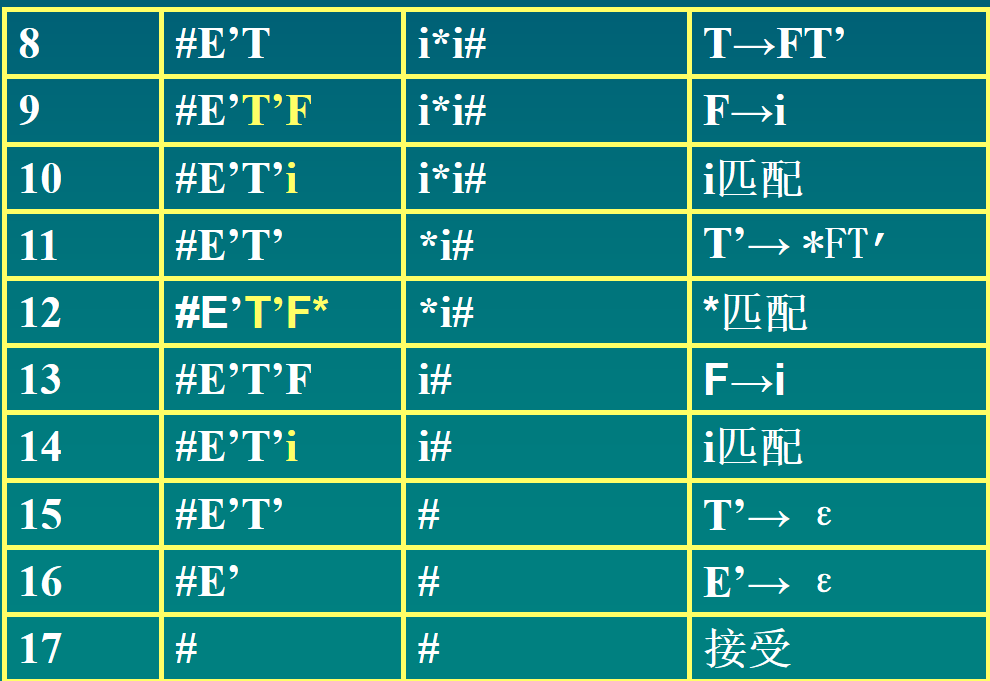
\includegraphics[scale = 0.3]{assets/CompilerConstructionPrinciples_1fd6a.png}
 \end{figure}

 递归子程序和预测分析法的对比:

 两者的思想是一致的,根据当前的状态来选取合适的产生式进行推导

 区别是递归下降子程序是利用递归程序的便利免除对环境的保存操作,而预测分析法则是手写栈保存过程中的记录。

 \section{LR分析法}
 \textbf{LR分析法}:根据当前分析栈种的符号串(通常以状态表示)和向右顺序查看输入串的K个($K\geq 0$)符号就可以唯一地确定句柄。

 \textbf{LR(k)}的含义:
 \begin{itemize}
  \item L表示从左到右扫描输入串
  \item R表示最左规约(即最右推到的逆过程)
  \item k表示向右查看输入符号串的个数
 \end{itemize}

 当$k=1$时,能满足当前绝大多数高级语言编译程序的需求

 \textbf{LR分析器的特点:}
 \begin{itemize}
  \item 是规范规约
  \item 适用范围广,适合于大多数上下文无关文法描述的语言
  \item 分析速度快,能准确定位错误
  \item 缺点:LR分析器的构造工作量大
 \end{itemize}

 \textbf{LR分析器的构成:}
 \begin{itemize}
  \item 总控程序\\
        所有LR分析器总共程序相同
  \item 分析表
        \begin{itemize}
         \item 不同文法有不同的分析表
         \item 同一文法采用的LR分析器不同,分析表也不同
         \item 分析表分为 \textbf{action表}(动作表) 和 \textbf{goto表}(状态转移表)
         \item GOTO表表示当前状态面临文法符号时应转向的下一个状态
         \item ACTION表 表示当前状态 面临 输入符号 时应采取的动作
        \end{itemize}
  \item 分析栈\\
        包括 \textbf{状态栈S} 和 \textbf{文法符号栈X}
 \end{itemize}

 \begin{figure}[H]
  \centering
  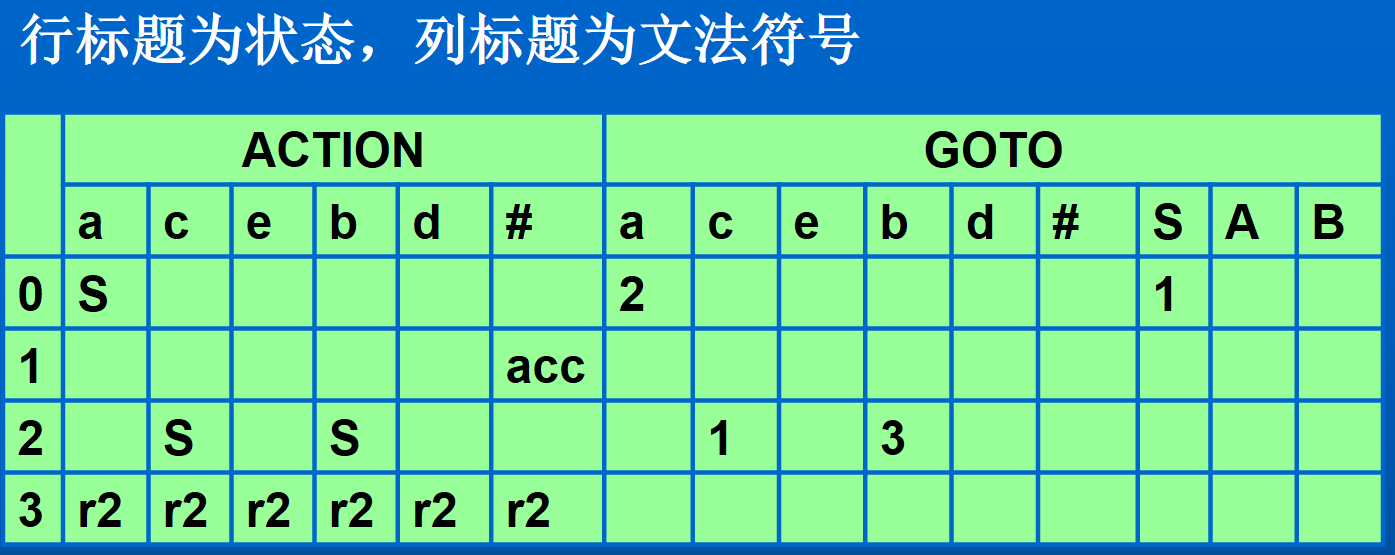
\includegraphics[scale = 0.3]{assets/CompilerConstructionPrinciples_e8d30.png}
  \caption{LR分析表}
 \end{figure}

 为节省空间:
 \begin{figure}[H]
  \centering
  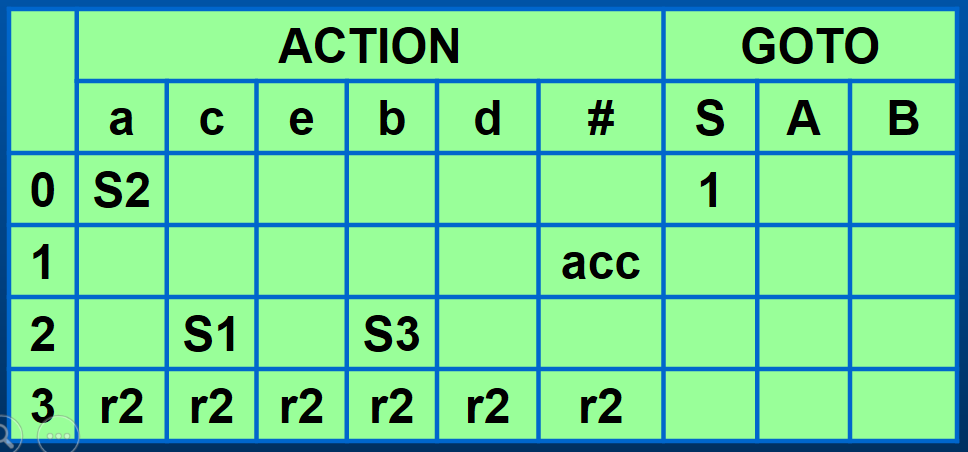
\includegraphics[scale = 0.3]{assets/CompilerConstructionPrinciples_a9086.png}
  \caption{LR分析表2}
 \end{figure}

 ACTION表 中的 动作 有4种:
 \begin{itemize}
  \item 移进$s_k$\\
        把状态$k$移入状态栈;\\
        若当前状态(未移入时的栈顶)是i,且 $k = GOTO[i,a]$ , 把a移入符号栈\\
        注:状态栈栈顶为当前状态;k为转移的状态,如果k为空的话,则报错
  \item 归约 $r_k$\\
        用第$k$条产生式进行归约,此时栈顶形成了句柄$\beta$,文法中第$k$条产生式为
        $A \to \beta$ , 且$|\beta| = r$\\
        归约时从状态栈和符号栈弹出$r$个符号,把$A$移入符号栈,$j = GOTO[i,A]$移入状态栈,其中状态$i$为修改后的栈顶状态
  \item 接受(acc)\\
        当符号栈只剩下文法开始符S,并且当前输入符为 \textbf{\#} , 则分析成功
  \item 报错\\
        当状态栈顶的状态遇到了不应该出现的文法符号,则报错,说明输入串不是该文法的句子
 \end{itemize}

 \subsection{LR(0)文法}
 \begin{itemize}
  \item LR(0) 分析器在分析的过程中只根据符号栈的内容就能确定句柄,不需要向右查看输入符号
  \item 对文法的限制较大, 对绝大多数高级语言的语法分析器不适用
  \item 构造LR(0)分析表的思想和方法是构造其他LR分析表的基础
 \end{itemize}

 LR(k)分析法通过 \textbf{活前缀来帮助确定句柄}
 \begin{itemize}
  \item 规范句型的可归约前缀和活前缀
  \item 构造文法的识别活前缀及可归前缀的DFA
  \item 按DFA构造相应分析表
  \item 按进行表进行$LR(k)$分析
 \end{itemize}

 \textbf{可归前缀:}规范句型中 \textbf{句柄之前} 包括 \textbf{句柄在内} 的串

 \textbf{活前缀}:形成 \textbf{可归前缀}之前(包括可归前缀在内)的所有规范句型的前缀,即规范句型的不含句柄右边符号的前缀。

 比如:规范句型$aAbcde$ 中,若$Ab$为句柄,则可归前缀为$aAb$,活前缀为:$\epsilon , a , aA , aAb$

 \textbf{可归前缀和活前缀在LR分析中的作用:}
 \begin{itemize}
  \item 在LR分析过程中,实际上是把 \textbf{活前缀} 列出放在符号栈中
  \item 一旦在栈中出现 \textbf{可归前缀} , 即 \textbf{句柄} 已经形成,就用相应的产生式进行归约
  \item 在分析的过程中,只要符号栈中的符号串是一个活前缀,就可保证已被分析过得部分是该文法规范句型的正确部分
 \end{itemize}

 使用 \textbf{DFA} 来识别前缀,为了构造这个DFA, 需要扩广文法

 \textbf{扩广文法:}使用$S'$作为文法的唯一开始,只要归约到$S'$即表示归约结束

 \textbf{扩广的原因:}文法开始符S可能出现在产生式的右部,在归约过程中,不能判断是归约到最后开始符,还是归约到在产生式右部出现的开始复,$S'$只出现在产生式的左部,确保不会混淆

 利用LR分析表分析步骤:
 \begin{itemize}
  \item 查找产生式的右部
  \item 左部将归约后的结果入栈
  \item ACC动作,分析结束
  \item 空白部分表示出错
 \end{itemize}

 问题:怎么得到LR分析表?LR分析表$\to$可归前缀$\to$DFA$\to$扩广文法+项目

 \spaceline
 \textbf{LR(0)项目}:在产生式的右侧适当位置添加一个小圆点,构成一个项目,小圆点后面部分表示待分析项

 比如:产生式$U\to XYZ$对应4个项目:$U\to \cdot XYZ,U\to X\cdot YZ,U\to XY\cdot Z,U\to XYZ\cdot $

 注:$A\to \epsilon$只有一个项目$A\to \cdot$

 项目的出现是为了标明当前所处的位置,以便后续的输入顺利进行。

 圆点的含义:
 \begin{itemize}
  \item 圆点在最左边,表示希望有产生式的右部归约
  \item 圆点在最右边,表示句柄已经形成,可以进行归约
  \item 圆点左部的内容,表示分析过程中已经识别过的部分
  \item 圆点右部的内容,表示待识别部分
 \end{itemize}

 项目分类:
 \begin{itemize}
  \item 移进项目,圆点后面为 \textbf{终结符}\\
        这个项下目输入a,表示移进操作
  \item 待约项目,圆点后面为 \textbf{非终结符}
  \item 归约项目,圆点在最右端\\
        表示句柄已经形成,在该项目下应该进行归约操作
  \item 接受项目:$S' \to S\cdot$
  \item 开始项目:$S' \to \cdot S$
 \end{itemize}

 \spaceline
 构造识别活前缀的NFA:
 \begin{itemize}
  \item 扩广文法
  \item 构造新状态,产生$LR(0)$项目\\
        所有项目为NFA的一个状态, 开始项目为初态,其他项目为活前缀的识别态(其中,归约项目为终态 , 接受项目为接受态)
  \item 确定状态的转换关系\\
        对于项目$i:A\to a\cdot Xb$ ,$j:A\to aX\cdot b$
        \begin{itemize}
         \item i和j连一条标记为X的箭弧
         \item 若X是非终结符($X\in V_N$), 对于X的所有产生式圆点在最左边的项目k , i和所有k 都连一条标记为$\epsilon$的箭弧
        \end{itemize}
  \item $NFA \to DFA$
 \end{itemize}

 整理:
 \begin{itemize}
  \item 考虑分析过程需要,引入项目的概念
  \item 随着分析过程,待归约串会发生变化,因而输入非终结符X需$X$和$\epsilon$两种弧(未识别出X的时候,走$
         \epsilon$,当识别出$X$时,走$X$弧)
 \end{itemize}

 \spaceline
 上述描述太过麻烦,工作量大,不实用,能否直接构造出$DFA$?
 解:可以,使用\textbf{项目集}作为$DFA$的状态

 运算:项目集 闭包,空串引发的子节点均合并到父节点上(实际上就是把上面$NFA\to DFA$的过程合并到创建过程上)

 \textbf{例:}
$S'\to E , E\to aA|bB,A\to cA | d , B\to cB | D$

$I = \{S' \to \cdot E\}$

 则$CLOSURE(I) = \{S'\to \cdot E , E\to \cdot aA , E\to \cdot bB\}$,为DFA的一个状态(因为后两条$\cdot$后面是非终结符,因此停止)

 \begin{figure}[H]
  \centering
  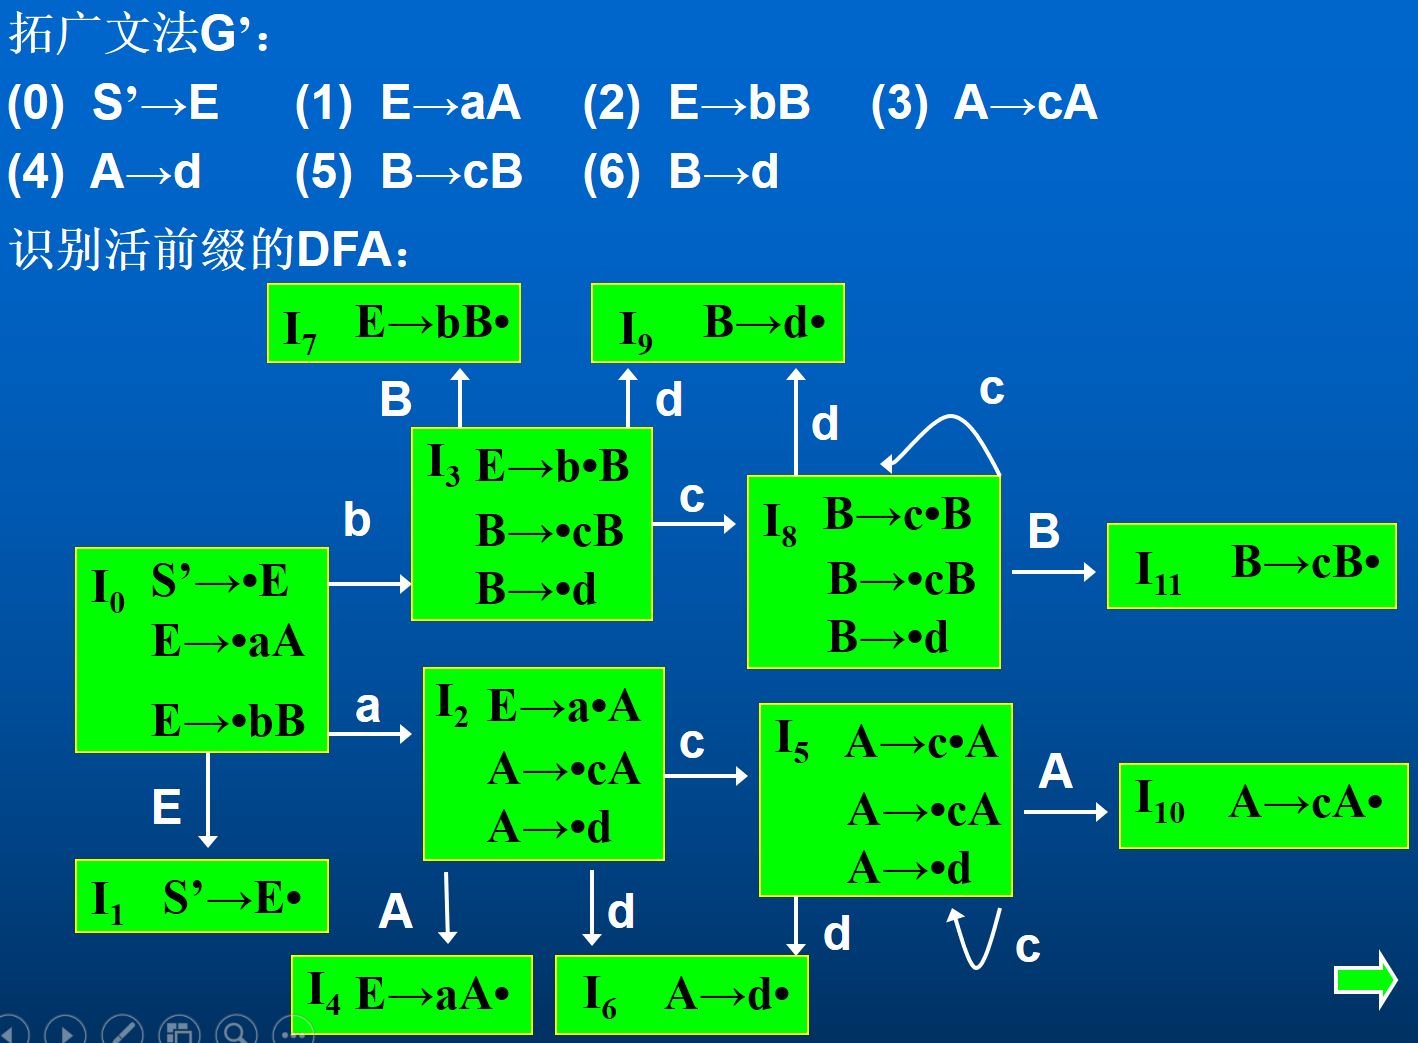
\includegraphics[scale = 0.3]{assets/CompilerConstructionPrinciples_30568.png}
  \caption{识别活前缀的DFA}
 \end{figure}

 \spaceline
 \textbf{LR(0)分析表的构造}:由$DFA$生成$LR(0)$分析表($S'\to \cdot S$表示初始状态)
 \begin{itemize}
  \item 输入终结符(LR(0)分析法要求这移进和归约操作不发生冲突)
        \begin{itemize}
         \item 如果项目集有归约项目,那么执行归约操作
         \item 否则执行移进操作
        \end{itemize}
  \item 输入非终结符,直接进行状态转移
 \end{itemize}

 问:如果当前的项目集既有归约项目进行归约,又能后续进行移进操作,怎么处理?SLR(0) , LR(1) ,LALR

 \begin{figure}[H]
  \centering
  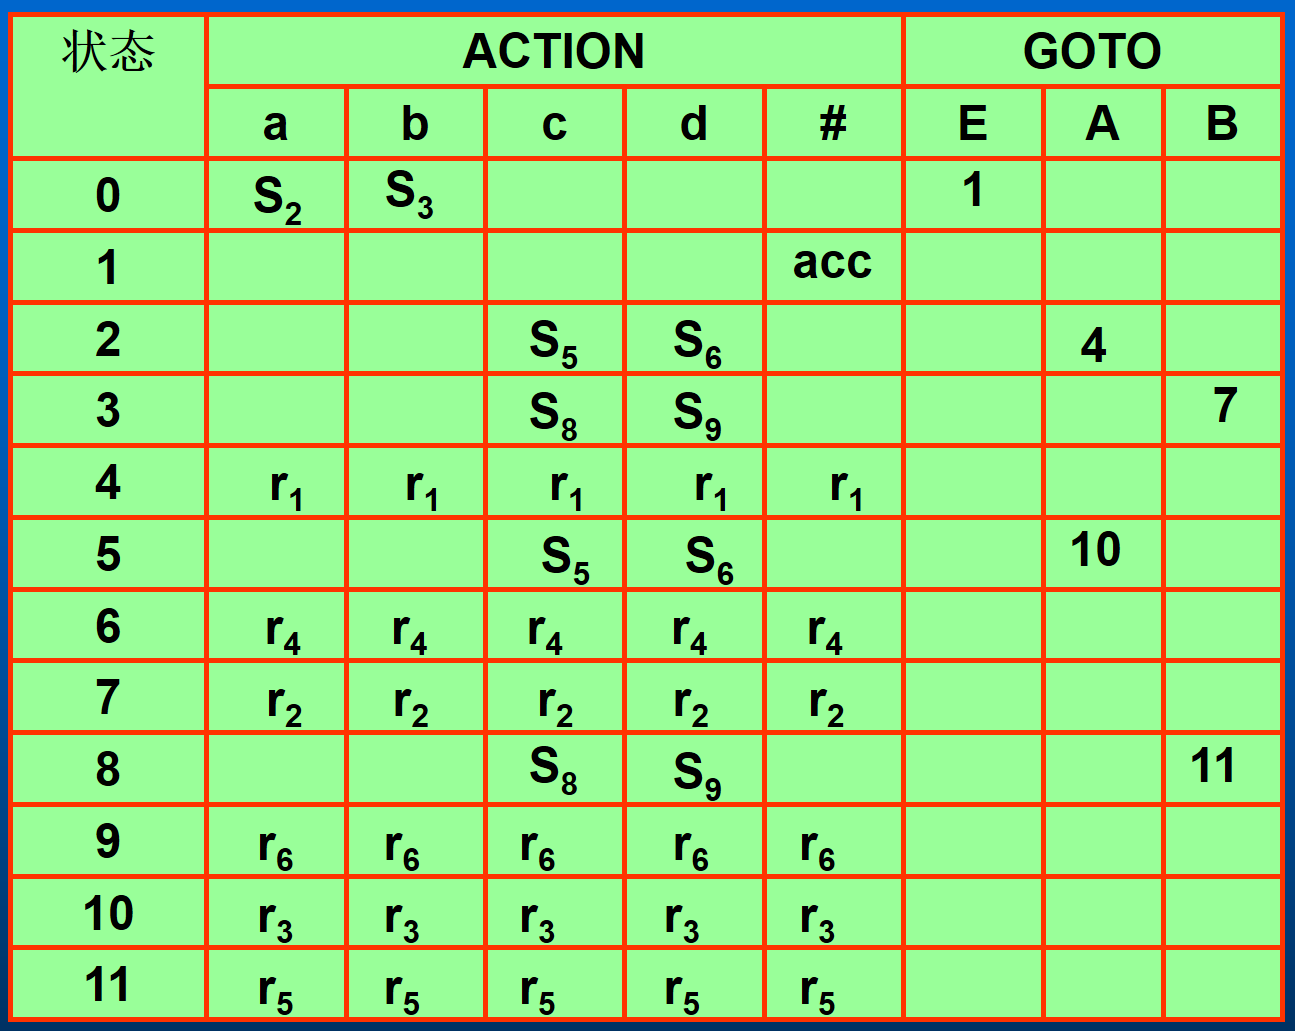
\includegraphics[scale = 0.3]{assets/CompilerConstructionPrinciples_dfa7c.png}
  \caption{从DFA构造LR(0)分析表}
 \end{figure}

 \spaceline
 \textbf{由LR(0)分析表分析过程:}查表$\to$状态转移$\to$acc或报错

 \begin{itemize}
  \item 移进$s_k$\\
        把状态$k$移入状态栈,若当前状态是i,且 $k = GOTO[i,a]$ , 把a移入符号栈
  \item 归约 $r_k$\\
        用第$k$条产生式进行归约,此时栈顶形成了句柄$\beta$,文法中第$k$条产生式为
        $A \to \beta$ , 且$|\beta| = r$\\
        归约时从状态栈和符号栈弹出$r$个符号,把$A$移入符号栈,$j = GOTO[i,A]$移入状态栈,其中状态$i$为修改后的栈顶状态
  \item 接受(acc)\\
        当符号栈只剩下文法开始符S,并且当前输入符为 \textbf{\#} , 则分析承购
  \item 报错\\
        当状态栈顶的状态遇到了不应该出现的文法符号,则报错,说明输入串不是该文法的句子
 \end{itemize}

 \begin{figure}[H]
  \centering
  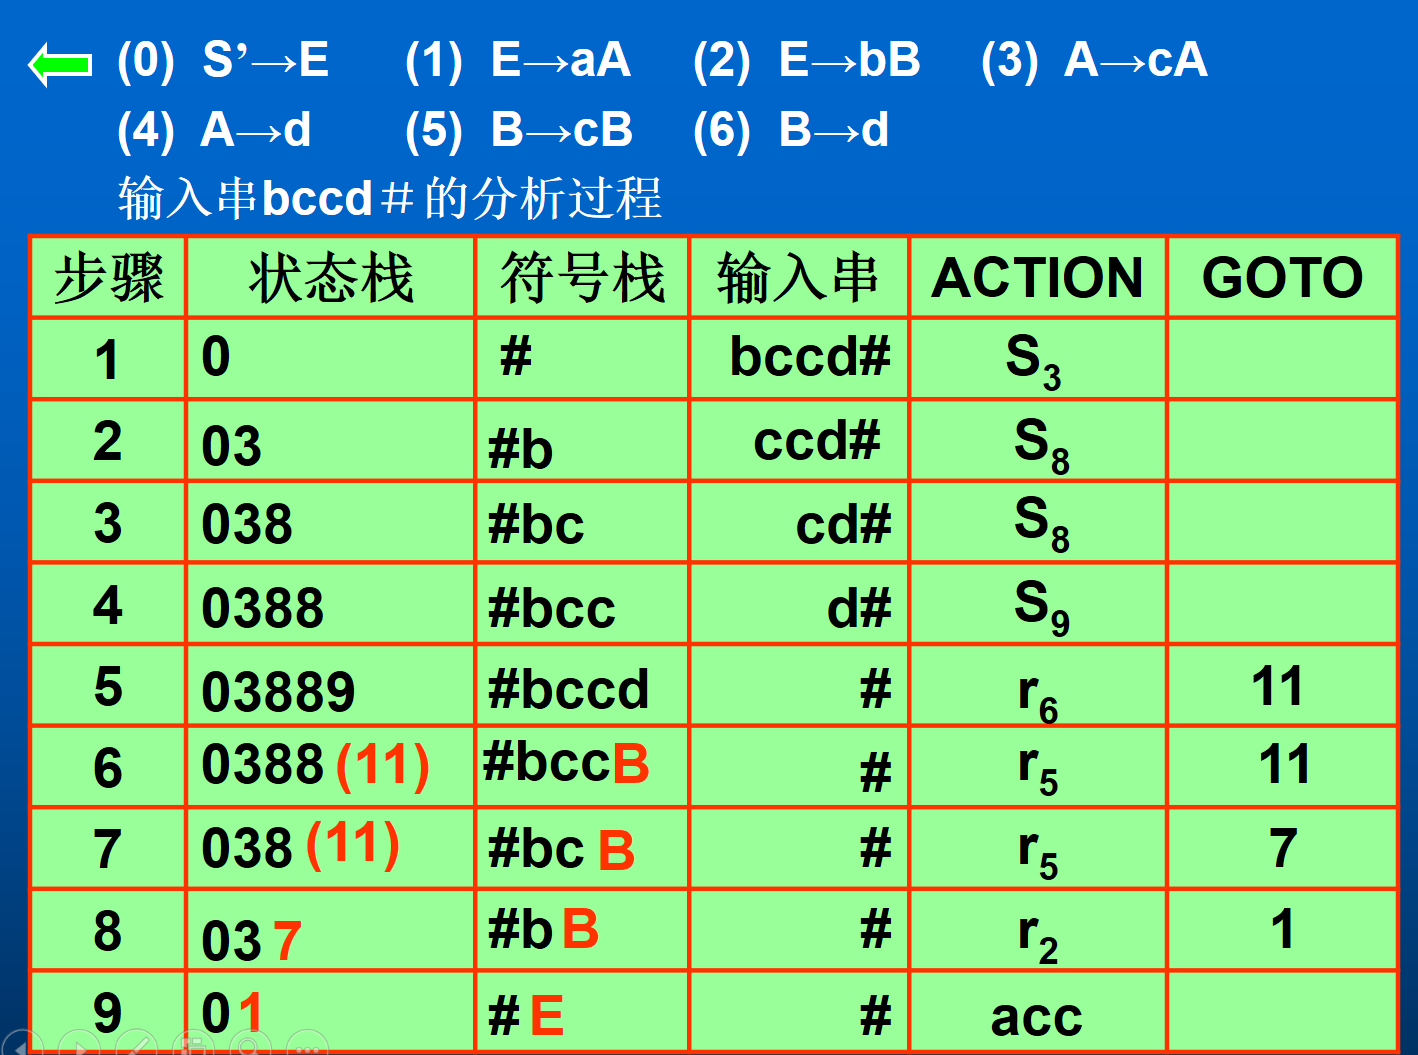
\includegraphics[scale = 0.3]{assets/CompilerConstructionPrinciples_a04e8.png}
  \caption{使用LR(0)分析表进行分析}
 \end{figure}

 \subsection{SLR(1)文法}
 文法可能存在'移进$\to$归约'和'归约$\to$归约'冲突

 \textbf{LR(0)文法:}项目集中既不存在'移进$\to$归约'也不存在'归约$\to$归约'冲突的文法

 \spaceline
 解决冲突的方法:使用$SLR(1)$文法:向前看一个输入符号,对于归约项目$A\to r \cdot$只有当后面的输入符号$a$,满足$a \in FOLLOE(A)$时才使用A的产生式进行归约

 \textbf{例:}对于$I = \{A\to a\cdot bc , A\to r \cdot , B\to e\cdot \}$

 \textbf{若$\{b\},FOLLOW(A) , FOLLOW(B)$两两不相交},当状态$I$面临输入符$a$时可采取以下动作:
 \begin{itemize}
  \item 若$a = b$ , 移进
  \item 若$a\in FOLLOW(A)$,则用$A\to r$归约
  \item 若$a\in FOLLOW(B)$,则用$B\to e$归约
  \item 否则,报错
 \end{itemize}

 \spaceline
 \textbf{例子:}P156 练习题T1 ,手机图片

 \subsection{LR(1)文法}
 SLR文法并不能完全解决冲突问题,因此需要进一步判断($LR(1)$文法)

 \spaceline
 \textbf{基本思想:}
 \begin{figure}[H]
  \centering
  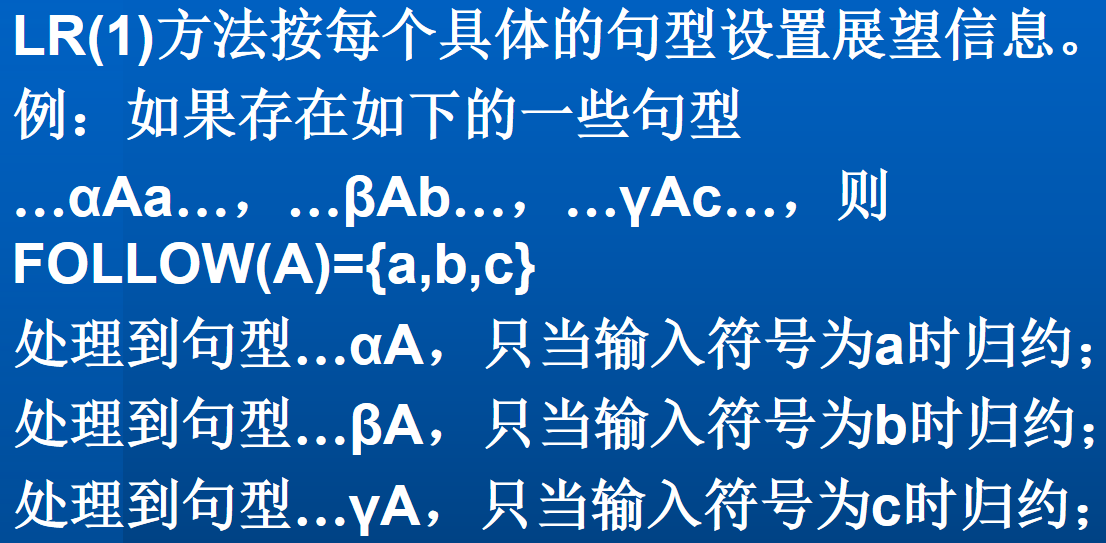
\includegraphics[scale = 0.3]{assets/CompilerConstructionPrinciples_3b12f.png}
  \caption{LR(1)分析的基本思想}
 \end{figure}

 \spaceline
 \textbf{LR(1)文法}:
 对于产生式:$A\to\alpha B \beta$,除了看$FOLLOE(B)$之外,还要看$FIRST(\beta)$,并把$First(\beta)$作为项目集的一个部分,通过这样进一步缩小可归约的范围

 \begin{figure}[H]
  \centering
  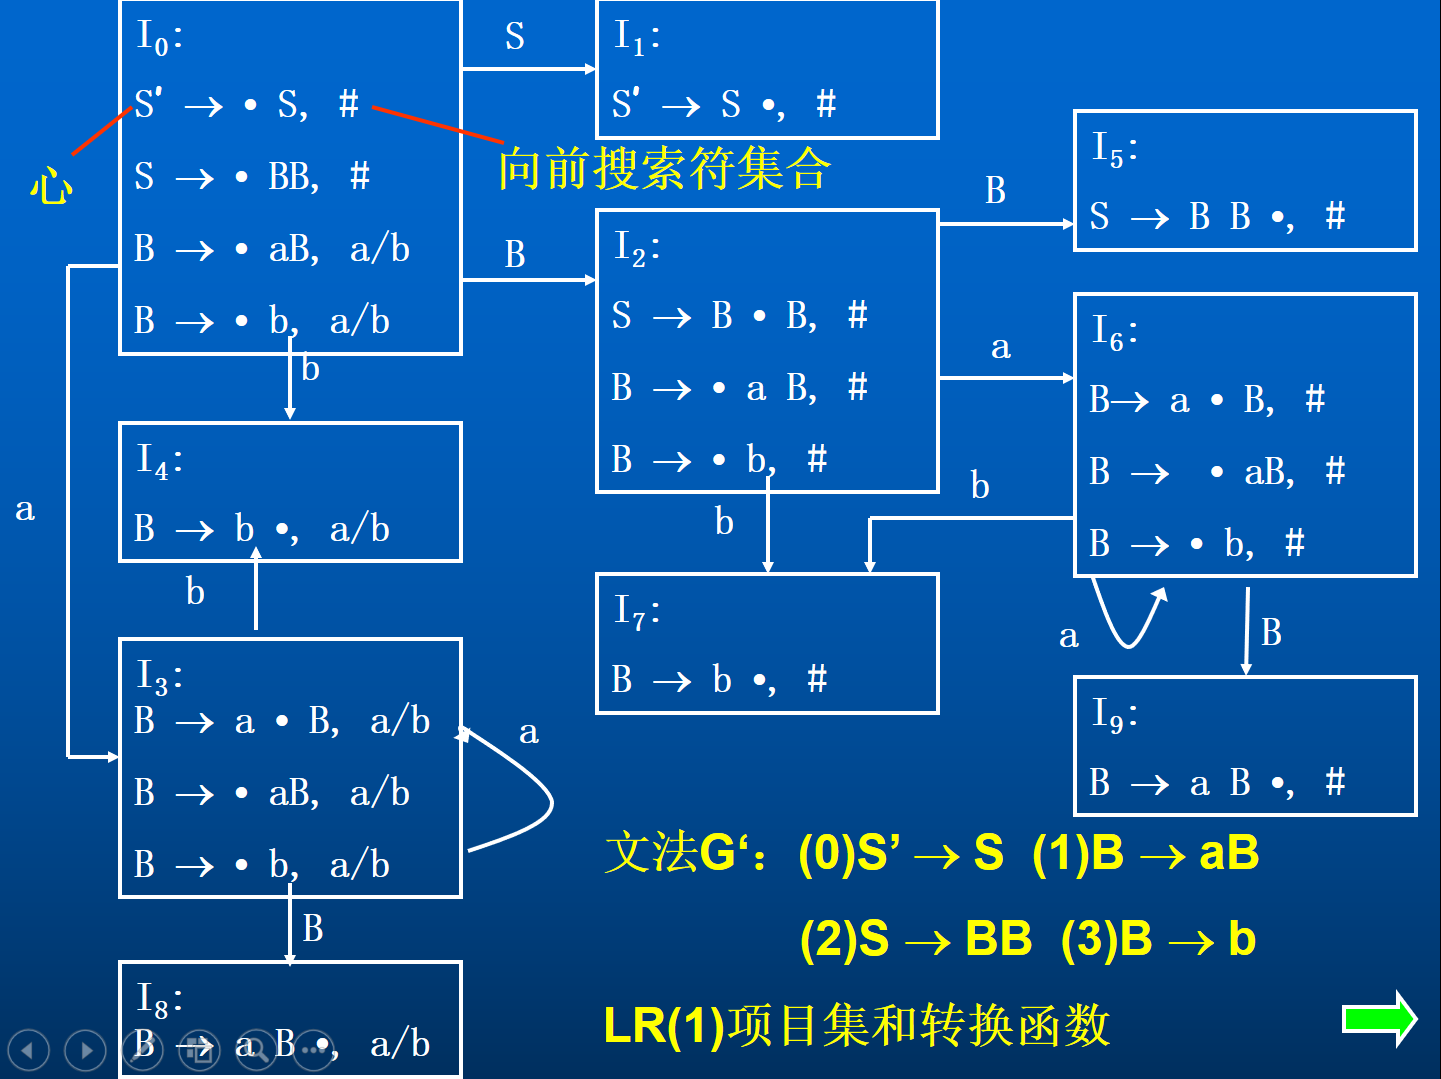
\includegraphics[scale = 0.3]{assets/CompilerConstructionPrinciples_87792.png}
  \caption{LR(1)分析的DFA}
 \end{figure}

 \spaceline
 \textbf{LR(1)文法的优点:}使用广度大

 \textbf{LR(1)文法的缺点:}LR(1)文法的状态数目庞大

 \subsection{LALR(1)文法}
 LALR(1)文法:$LR(1)$的状态数目太过庞大,不好计算,只有在$SLR(1)$文法无法解决问题的部分,才采用$LR(1)$文法进行解决。

 \section{中间代码生成}
 \subsection{属性文法}
 \textbf{属性:}对文法的每个符号,引进一些属性,这些属性代表与文法符号相关的信息,如类型、值、存储位置等

 \textbf{语义规则:}为文法的每个产生式配备的计算属性的计算规则

 \textbf{属性文法}:带属性的文法

 \textbf{例:}$E\to A + B \{A.t = int \quad AND \quad B.t = int\}$

 (花括号内为$E$的语义规则)

 \textbf{属性分类:}
 \begin{itemize}
  \item 综合属性\\
        属性值由该节点的子节点的属性值计算来\\
        用于自下而上传递信息
  \item 继承属性\\
        属性值由该节点的兄弟节点或父节点的属性值计算而来\\
        用于自上而下传递信息\\
        终结符只有综合属性,他们由词法分析器提供\\
        非终结符既有综合属性也有继承属性,但文法开始符没有继承属性
 \end{itemize}

 \subsection{语法制导的翻译}
 基本思想:在语法分析过程中,随着分析的步步进展,每当使用一条产生式进行推导或归约,就执行该产生式所对应的语义动作,完成相应的翻译工作

 语法制导翻译法不论对自上而下还是自下而上的分析都适用

 一旦语法分析确认输入符号串是一个句子,它的值也同时由语义规则计算出来

 对于LR分析(自下而上)的语法分析来说,在归约后调用语义规则的功能需要增加予以栈,语义值放到与符号栈同步操作的语义栈中,多项语义值可设多个语义栈

 栈结构格式为:
 \begin{figure}[H]
  \centering
  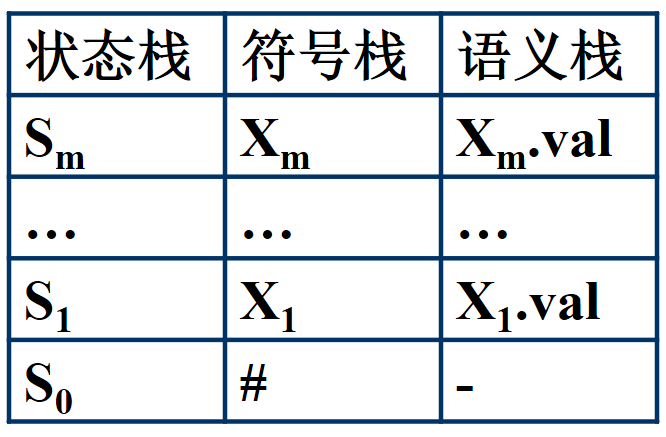
\includegraphics[scale = 0.3]{assets/CompilerConstructionPrinciples_c4498.png}
  \caption{LR分析栈结构}
 \end{figure}

 例:
 \begin{figure}[H]
  \centering
  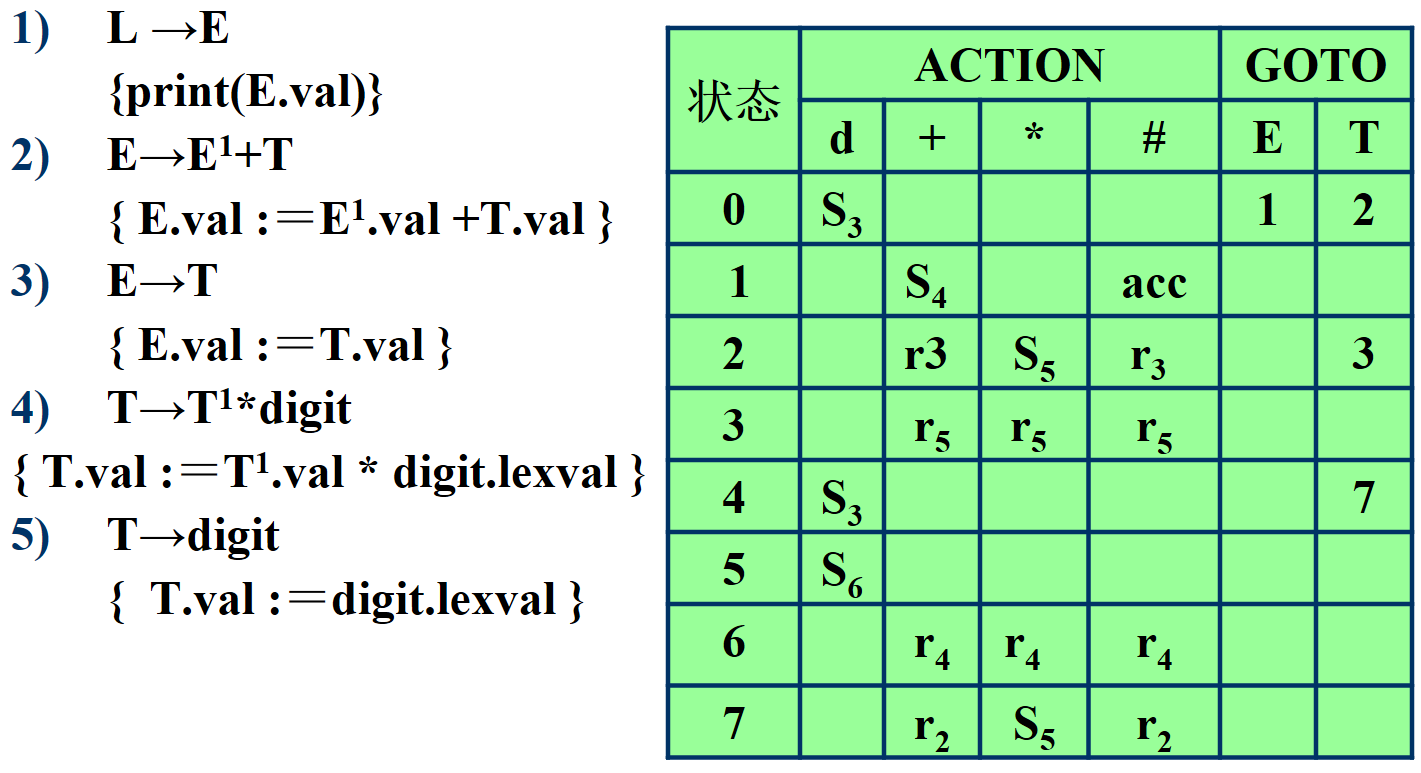
\includegraphics[scale = 0.3]{assets/CompilerConstructionPrinciples_443d1.png}
  \caption{简单算数表达式求值的属性文法}
 \end{figure}

 \begin{figure}[H]
  \centering
  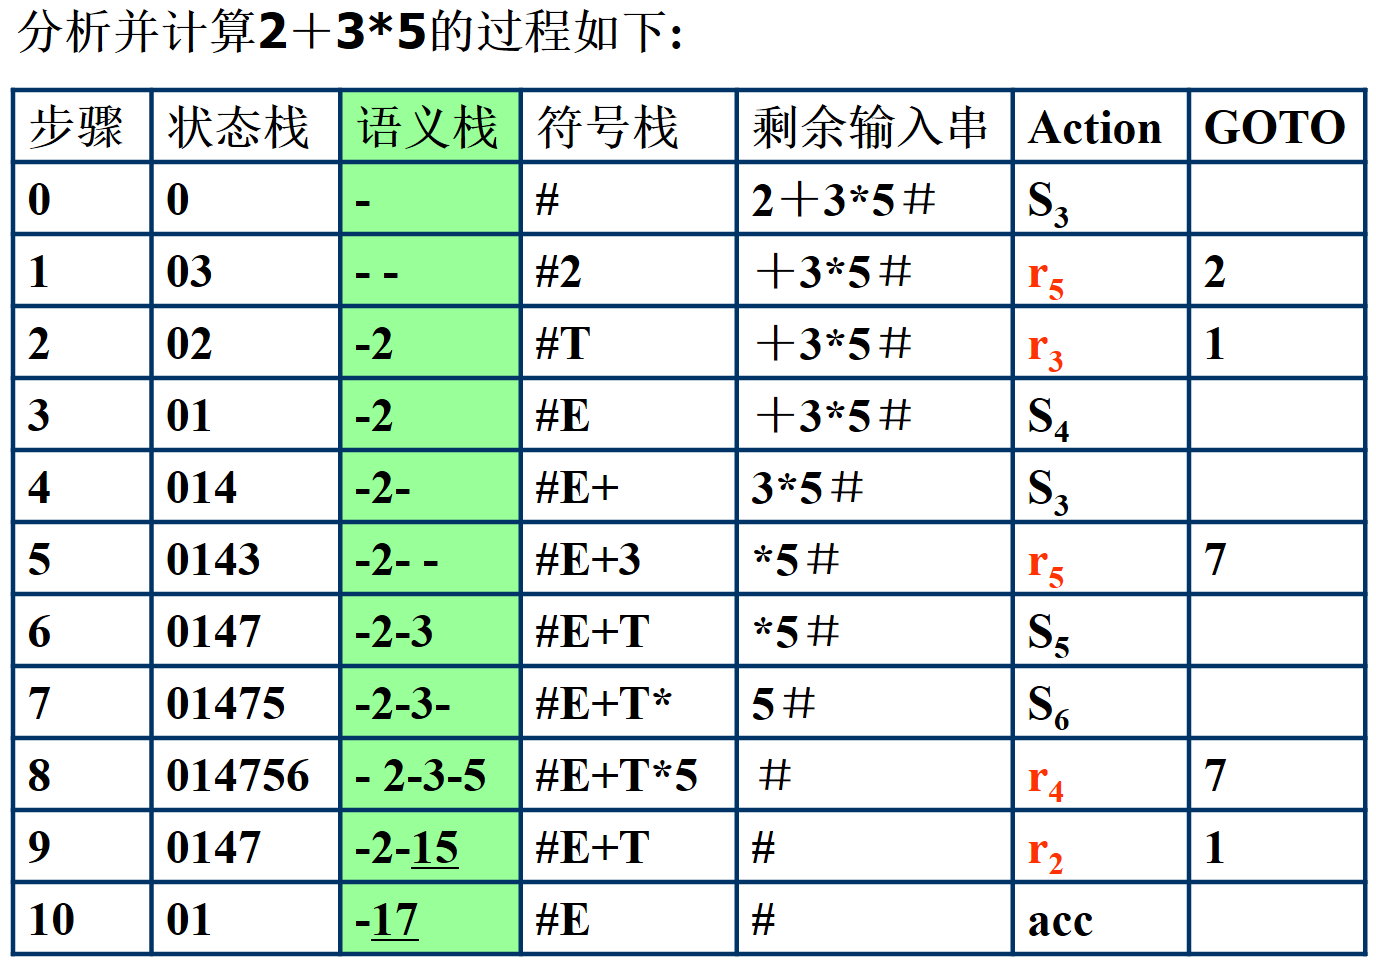
\includegraphics[scale = 0.3]{assets/CompilerConstructionPrinciples_4966b.png}
  \caption{计算2+3*5}
 \end{figure}

 \subsection{中间代码}

 \textbf{中间代码:}
 中间代码是一种复杂性介于源程序语言和机器语言之间的一种表示形式,与具体机器无关,可以进行与机器无关的优化

 \textbf{中间代码的形式:}
 \begin{itemize}
  \item 逆波兰记号\\
        也叫后缀式,运算对象写在前面
  \item 三元式
  \item 四元式
  \item 树
 \end{itemize}

 \subsection{中间代码生成}
 属性和语义规则中用到的变量、过程和函数:

 属性:
 \begin{itemize}
  \item id.name\\
        表示单词id的名字
  \item E.place\\
        表示存放E值的变量名在符号表的入口地址或临时变量编码
 \end{itemize}

 变量、函数和过程:
 \begin{itemize}
  \item nextstat\\
        给出在输出序列中下一个四元式的序号
  \item lookup(id.name)\\
        查询id.name是否出现在符号表中,是则返回id的入口地址,否则返回nil
  \item emit\\
        向输出序列输出一个四元式\\
        emit每调用一次,nextstat的值增加1
  \item newtemp\\
        生成一个新的临时变量
  \item error\\
        进行错误处理
 \end{itemize}

 \subsubsection{简单赋值语句的翻译}
 语义主要审查标识符是否已经声明
 \begin{itemize}
  \item \begin{figure}[H]
         \centering
         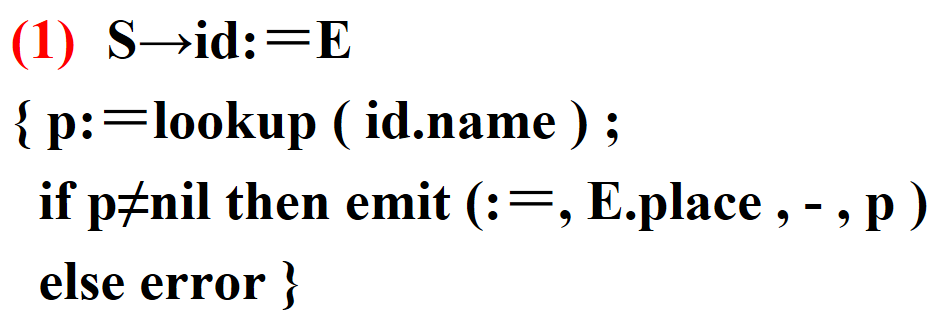
\includegraphics[scale = 0.3]{assets/CompilerConstructionPrinciples_733a7.png}
        \end{figure}
  \item \begin{figure}[H]
         \centering
         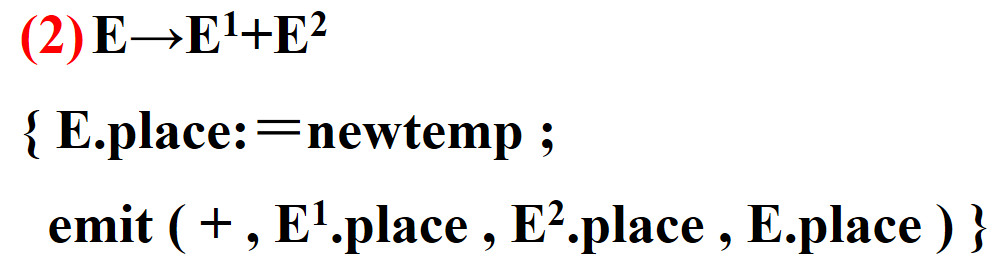
\includegraphics[scale = 0.3]{assets/CompilerConstructionPrinciples_74c0a.png}
        \end{figure}
  \item \begin{figure}[H]
         \centering
         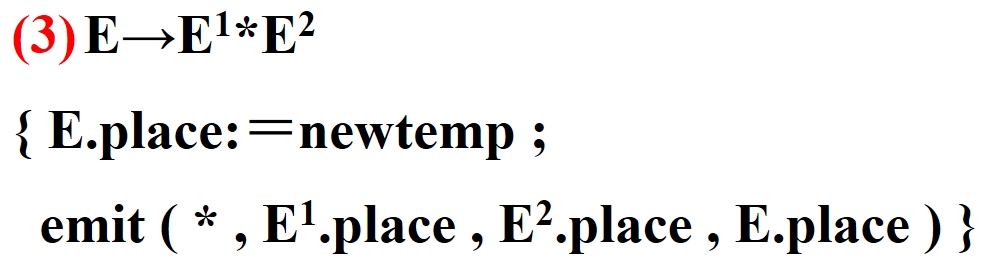
\includegraphics[scale = 0.3]{assets/CompilerConstructionPrinciples_f88bc.png}
        \end{figure}
  \item \begin{figure}[H]
         \centering
         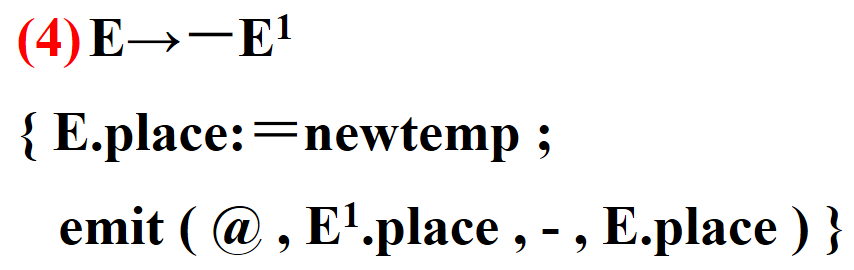
\includegraphics[scale = 0.3]{assets/CompilerConstructionPrinciples_45864.png}
        \end{figure}
  \item \begin{figure}[H]
         \centering
         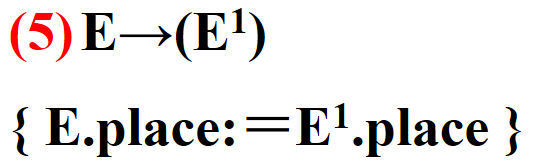
\includegraphics[scale = 0.3]{assets/CompilerConstructionPrinciples_4cdaf.png}
        \end{figure}
  \item \begin{figure}[H]
         \centering
         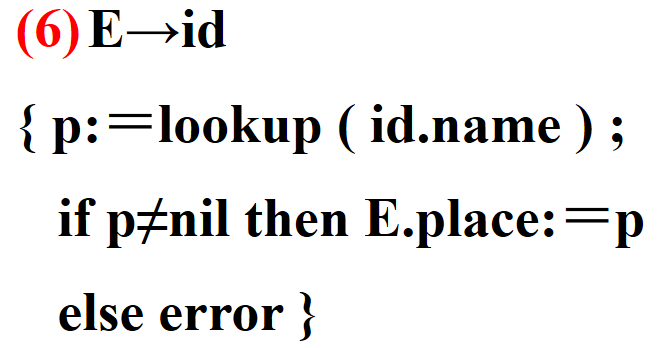
\includegraphics[scale = 0.3]{assets/CompilerConstructionPrinciples_75972.png}
        \end{figure}
 \end{itemize}

 \subsubsection{布尔表达式的翻译}
 \textbf{直接翻译:}把结果保存在临时变量,对于比较运算,则采用赋值语句进行结果的赋值
 \begin{figure}[H]
  \centering
  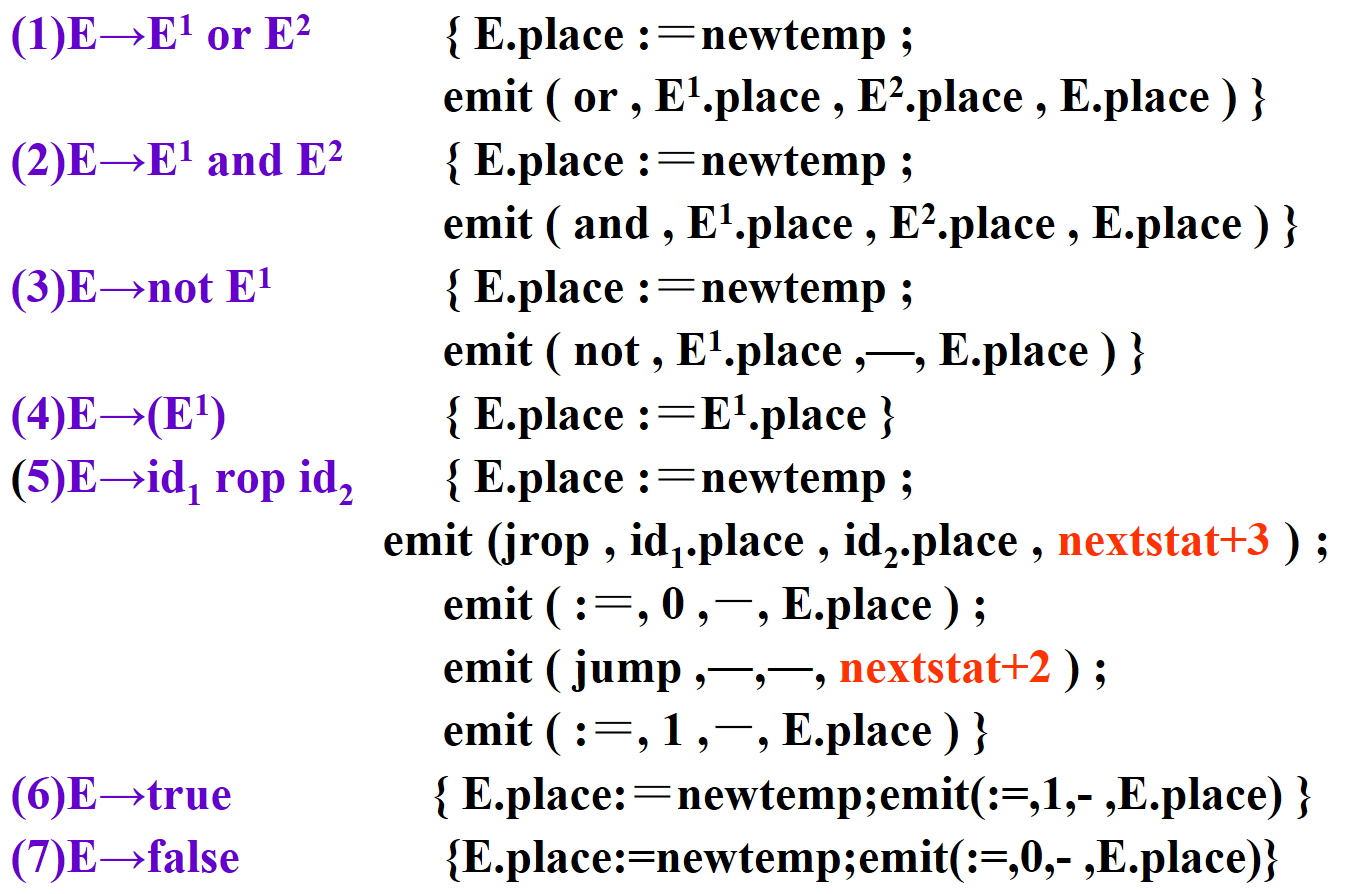
\includegraphics[scale = 0.3]{assets/CompilerConstructionPrinciples_e815e.png}
 \end{figure}

 \textbf{短路翻译:}对于布尔表达式,一旦确定了真假,就无需进行后续的判断,直接进行跳转即可

 主要有以下3种代码:
 \begin{figure}[H]
  \centering
  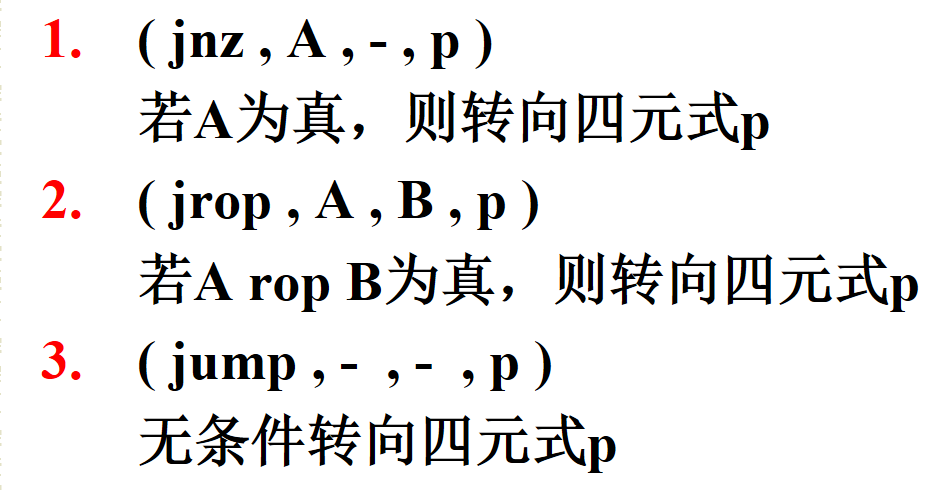
\includegraphics[scale = 0.3]{assets/CompilerConstructionPrinciples_36d92.png}
 \end{figure}

 对于$a\quad rop\quad b$形式,生成以下代码:
 \begin{figure}[H]
  \centering
  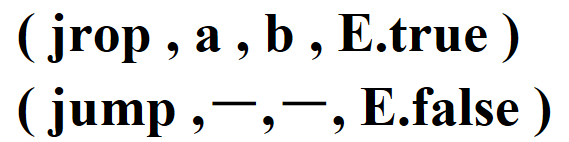
\includegraphics[scale = 0.3]{assets/CompilerConstructionPrinciples_7394b.png}
 \end{figure}

 但是,在翻译E的时候,我们并不能确定两个跳转语句将要跳转的位置,
 因此我们需要保存这两条四元式的序号,以便生成完后续的代码之后进行回填

 \begin{itemize}
  \item E.true \\
        是一个链表,E的中间代码中,判断E为"真"时发生跳转的四元式的编号
  \item E.false \\
        是一个链表,E的中间代码中,判断E为"假"时发生跳转的四元式的编号
 \end{itemize}

 为了完成翻译过程:我们定义以下过程和变量:
 \begin{itemize}
  \item merge(p1,p2)\\
        把p1和p2为链首的两条链,并返回合并后的链首
  \item backpatch(p,t)\\
        把链首p所连接的每个四元式的第四区段填为转移目标t
  \item E.codebegin\\
        表示E的第一个四元式的序号
 \end{itemize}

 \begin{figure}[H]
  \centering
  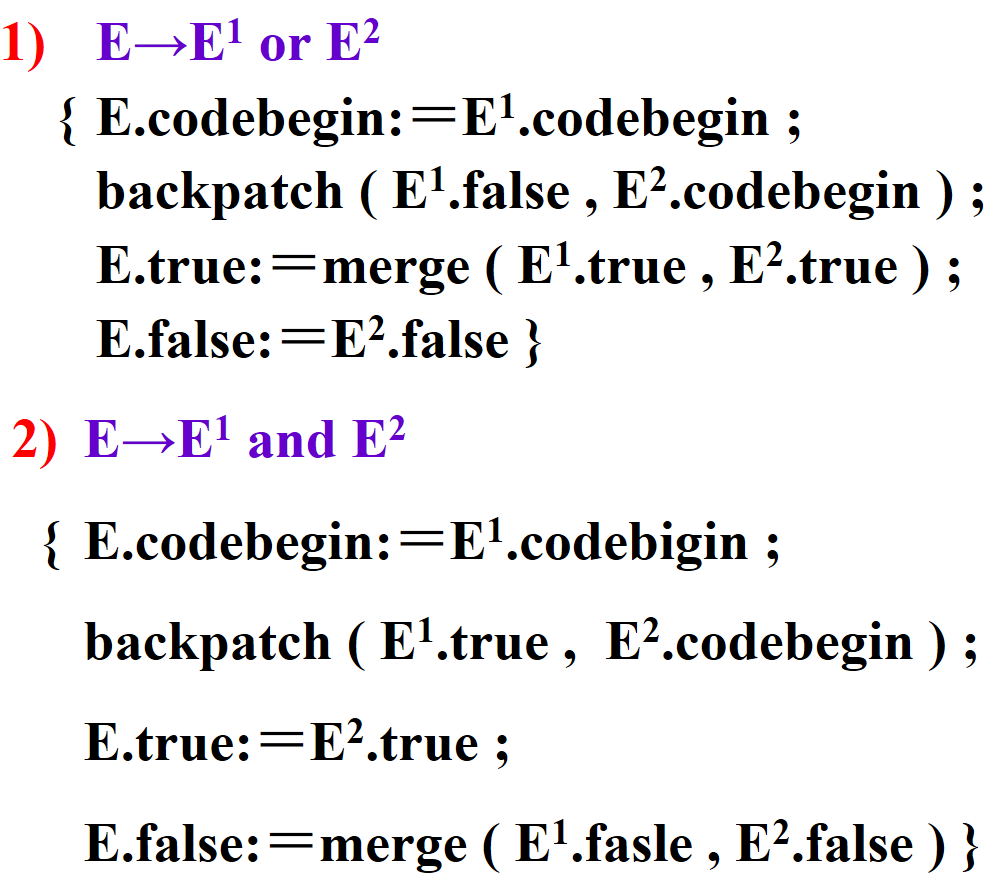
\includegraphics[scale = 0.3]{assets/CompilerConstructionPrinciples_859b6.png}
 \end{figure}

 \begin{figure}[H]
  \centering
  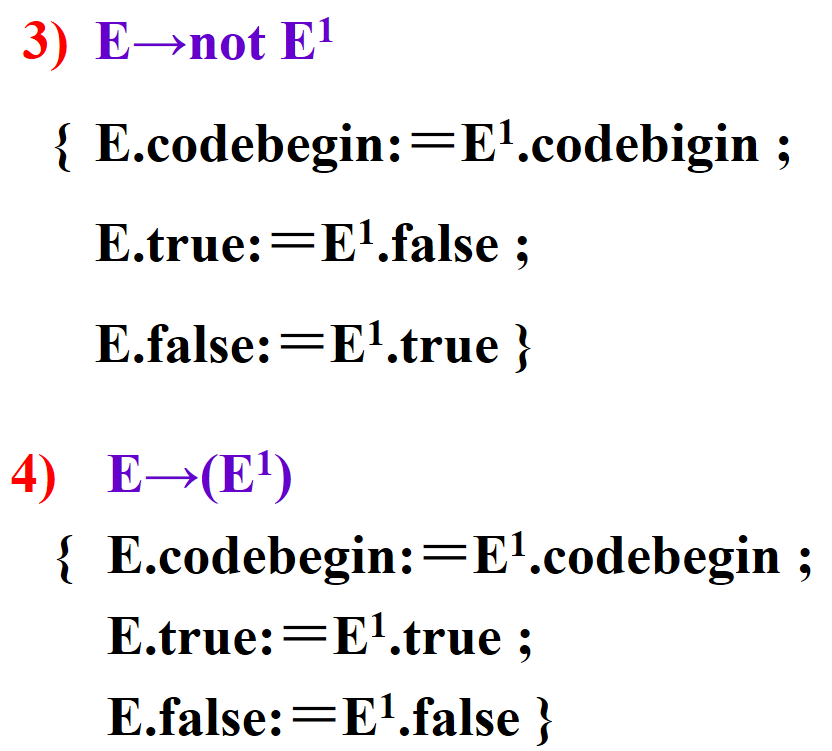
\includegraphics[scale = 0.3]{assets/CompilerConstructionPrinciples_844ba.png}
 \end{figure}

 \begin{figure}[H]
  \centering
  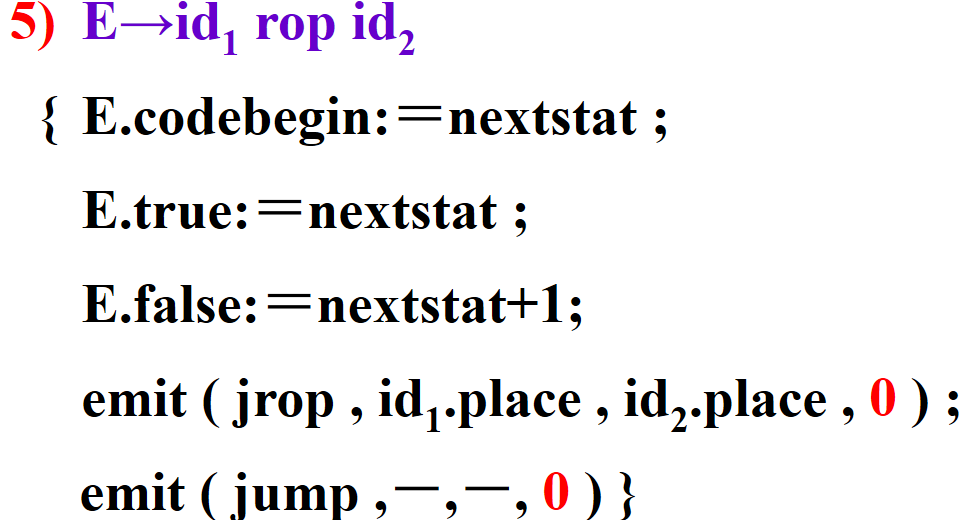
\includegraphics[scale = 0.3]{assets/CompilerConstructionPrinciples_38961.png}
 \end{figure}

 \begin{figure}[H]
  \centering
  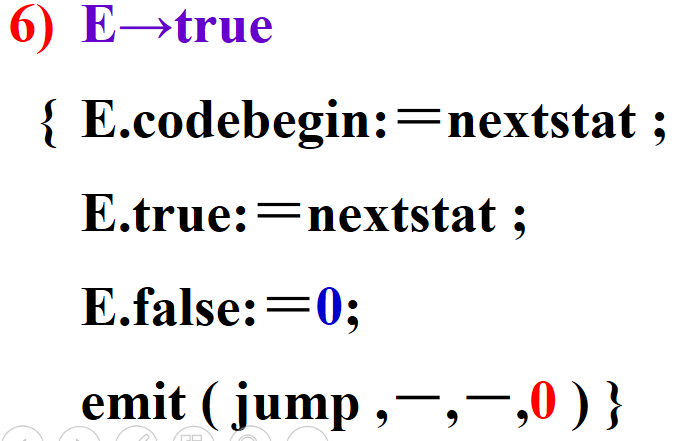
\includegraphics[scale = 0.3]{assets/CompilerConstructionPrinciples_4c318.png}
 \end{figure}

 \begin{figure}[H]
  \centering
  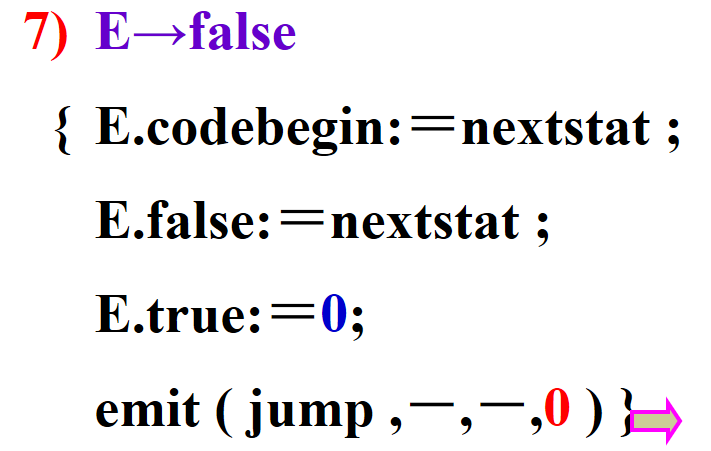
\includegraphics[scale = 0.3]{assets/CompilerConstructionPrinciples_f65f3.png}
 \end{figure}

 \subsubsection{if,while,repeat 语句的翻译}
 \begin{figure}[H]
  \centering
  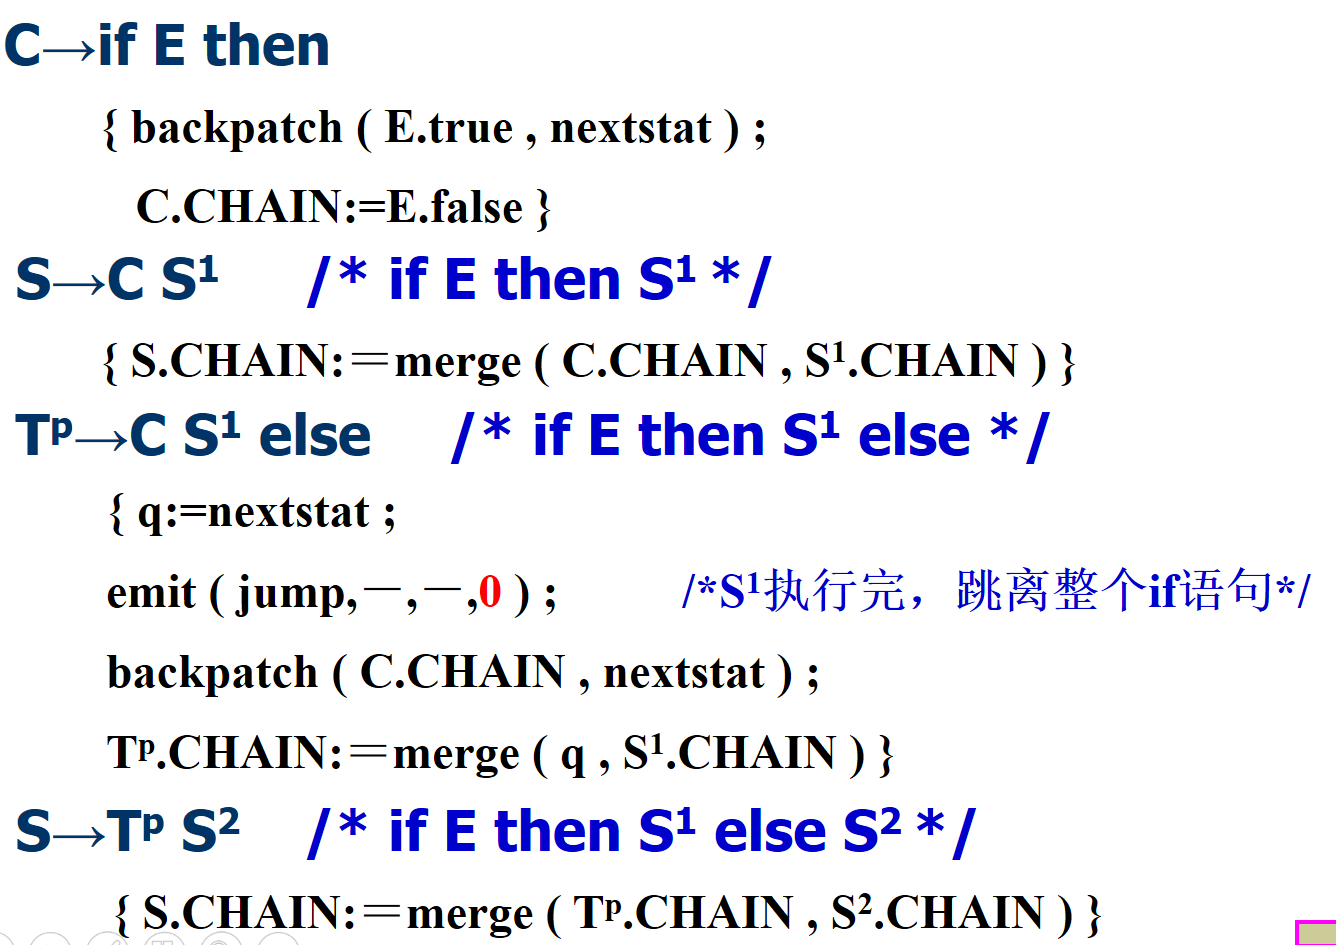
\includegraphics[scale = 0.3]{assets/CompilerConstructionPrinciples_d0192.png}
 \end{figure}

 \begin{figure}[H]
  \centering
  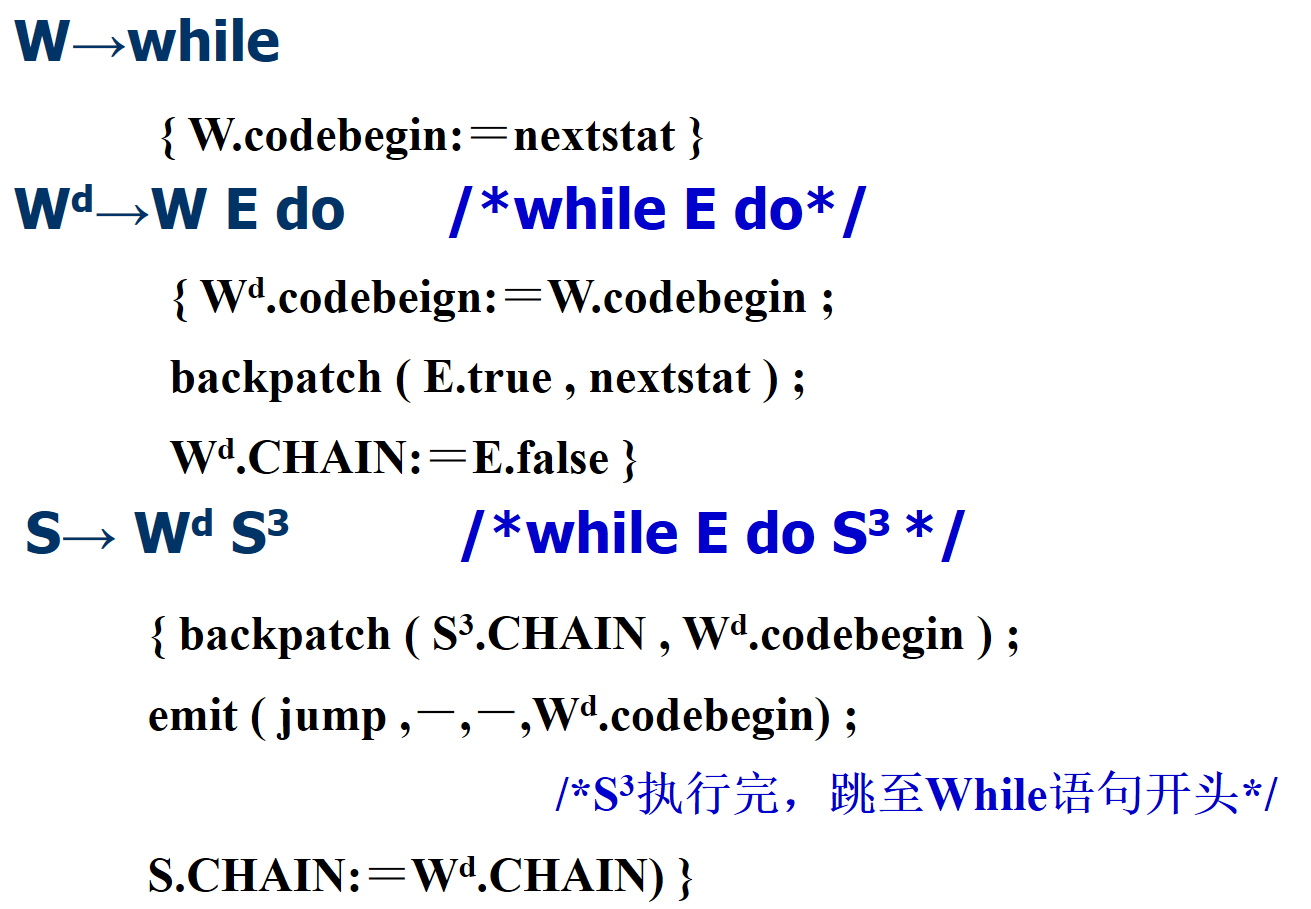
\includegraphics[scale = 0.3]{assets/CompilerConstructionPrinciples_ba2f4.png}
 \end{figure}

 \textbf{C.chain}的含义:表示C的四元式中,跳转到C的代码块末尾(出口)的四元式的集合

 实际上,$E.true$和 $E.false$已经能够翻译出语句了,但是为什么还需要$C.chain$?

\begin{itemize}
  \item 对于语句嵌套的时候,如果没有回填$chain$,那么就需要经过 \textbf{多次跳转}才能跳到出口
  \item 在 $if$ 语句中,$then$ 代码块结束之后,需要跳过$else$的代码块,如果使用$chain$之后,就不需要在$if$的子程序里面对这个$jmp$进行填写
\end{itemize}


比如:以下代码
while E do
\quad if A then B

在while结束的时候,会有一条 \textbf{jmp1}语句跳转到while语句的开头

在 \textbf{if}语句为false的时候,会有 \textbf{jmp2} 跳转到 if语句块的结束,也就是 \textbf{jmp1} 语句,再由jmp1跳转到while开头(\textbf{注意,这里jmp了两次})

由chain的定义,我们可以知道 \textbf{$IF.chian = jmp2$} , 也就是前图中的 \textbf{$S^3.chain = jmp2$}

我们 \textbf{回填} while.codebegin 到 \textbf{jmp2}的话,那么执行 \textbf{jmp2}的时候,就直接到了while 的开头,而无需再经过 \textbf{jmp1} (划重点:\textbf{回填chain后,只jmp了一次})

\textbf{例:}
\begin{figure}[H]
 \centering
 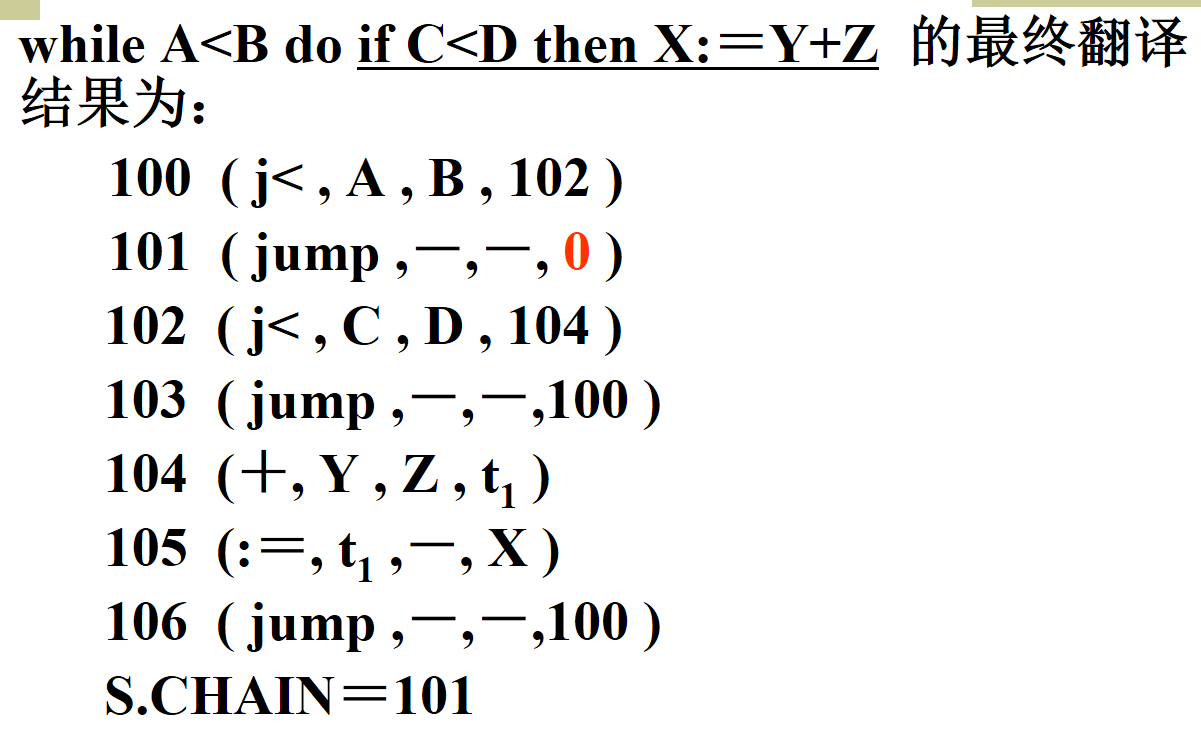
\includegraphics[scale = 0.3]{assets/CompilerConstructionPrinciples_1152a.png}
\end{figure}
\begin{figure}[H]
 \centering
 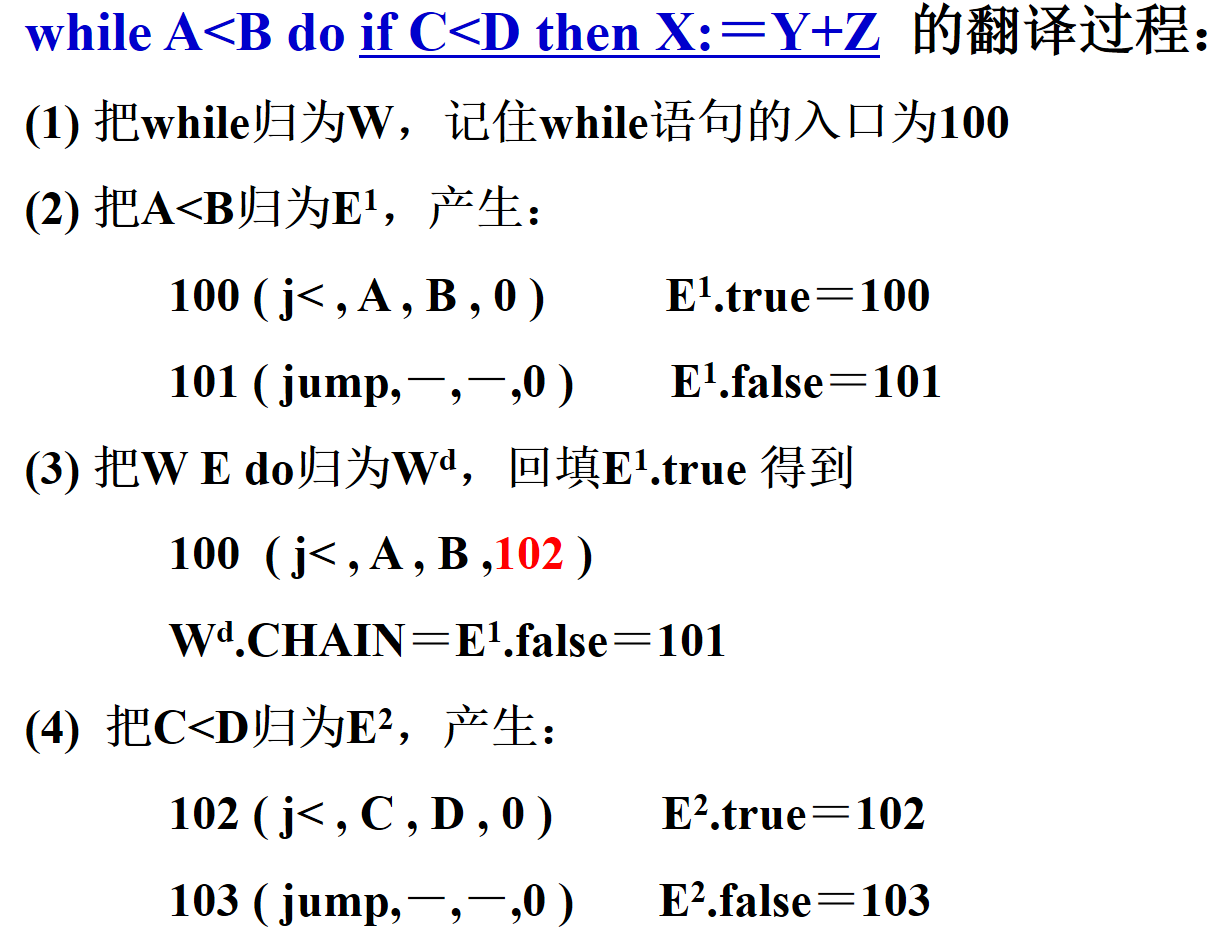
\includegraphics[scale = 0.3]{assets/CompilerConstructionPrinciples_b905b.png}
\end{figure}
\begin{figure}[H]
 \centering
 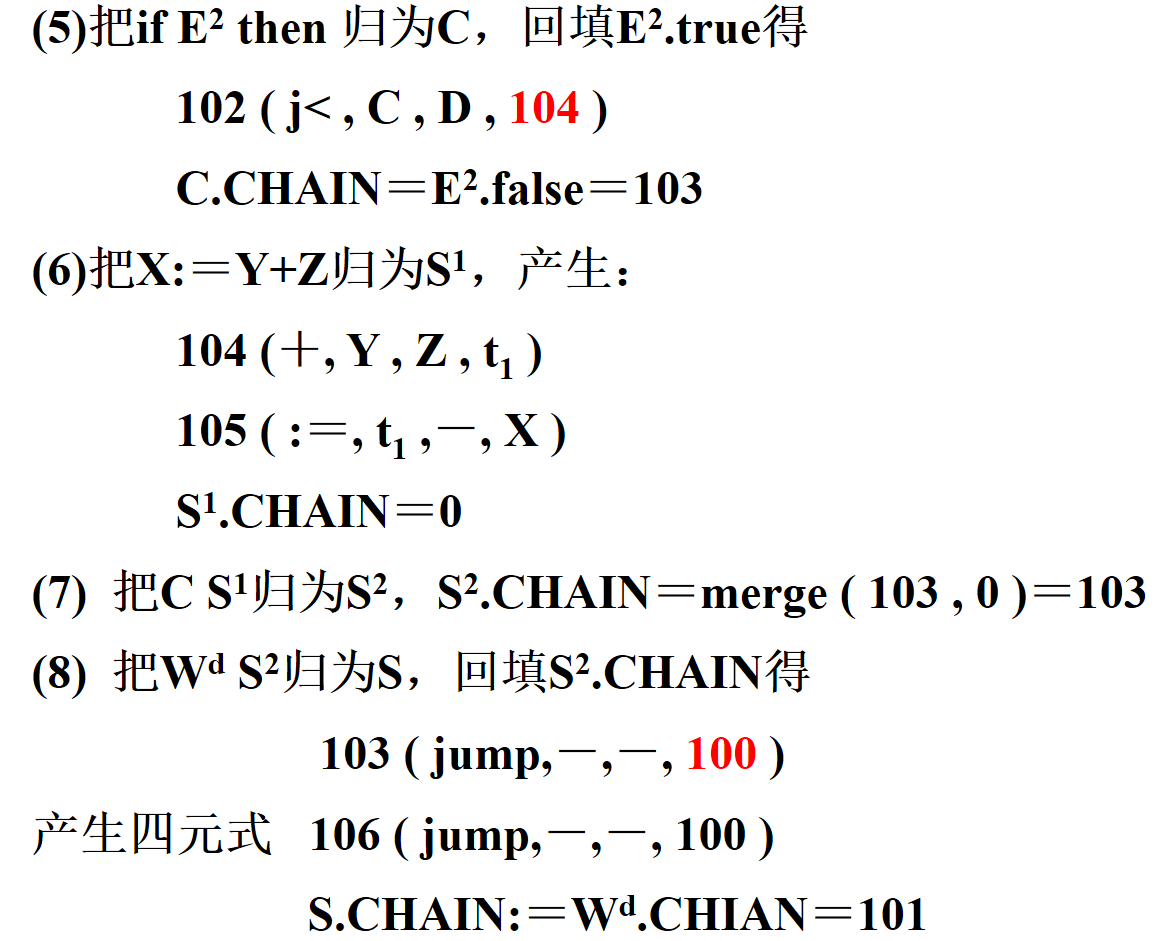
\includegraphics[scale = 0.3]{assets/CompilerConstructionPrinciples_8744b.png}
\end{figure}

\section{符号表}
\textbf{符号表}:符号表是存放标识符信息的一种表,其中的信息表示是标识符的属性(语义)

\textbf{符号表的作用:}符号表是连接声明和引用的桥梁。
\begin{itemize}
 \item 一个名字在声明时,相关信息被写进符号表
 \item 在引用时,根据符号表中的信息生成相应的可执行语句
\end{itemize}

\textbf{符号表的生存周期:}编译过程中,每当遇到标识符时,就要查填符号表
\begin{itemize}
 \item 若是新的标识符,就向符号表中填入一个新的表项
 \item 否则,根据情况向符号表中的已有表项 \textbf{增填} 信息(如填入分析的存储地址)或者 \textbf{查获}信息(如语义检查)

\end{itemize}

\section{代码优化}
\textbf{代码优化:}对代码进行等价变换,使得变换后的代码效率更高(节省运行时间、存储空间 或者两者兼而有之)

\begin{itemize}
 \item 中间代码优化(不依赖具体计算机)
 \item 目标代码优化(依赖具体计算机)
\end{itemize}

\begin{figure}[H]
 \centering
 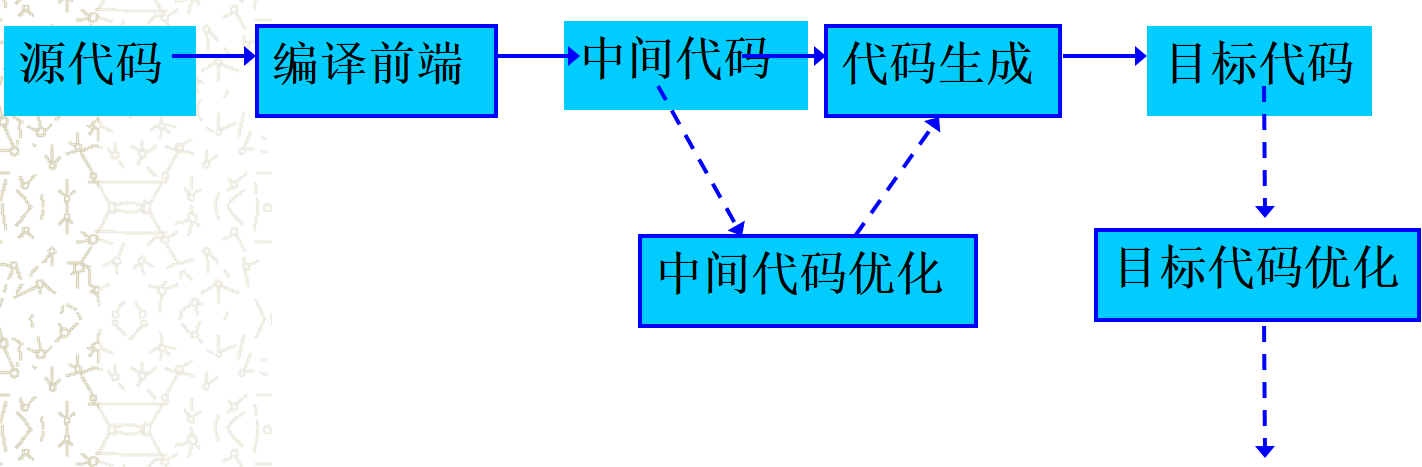
\includegraphics[scale = 0.3]{assets/CompilerConstructionPrinciples_9646f.png}
 \caption{编译的优化工作阶段}
\end{figure}

\textbf{优化的分类:}
\begin{itemize}
 \item 局部优化\\
       在只有一个入口、一个出口的基本快上进行优化
 \item 循环优化\\
       对循环中的代码进行优化
 \item 全局优化\\
       在整个程序范围内进行的优化
\end{itemize}

\subparagraph{中间代码优化}
\textbf{中间代码常用计数:}
\begin{itemize}
 \item 删除多余运算(删除公共子表达式)\\
       如果子表达式E在前面计算过,且之后E中的变量值都未改变,那么E的重复出现称为 \textbf{公共子表达式},可避免重复计算
 \item 合并已知量与复写传播\\
       如果运算量都是已知量,则在编译时就算出它的值,称 \textbf{合并已知量}\\
       若有$A:= B$,称为把B \textbf{复写}到A,如果其后有引用A的地方,且其间A、B的值都未改变,则可把对A的引用改为对B的引用,称为 \textbf{复写传播}
 \item 删除无用赋值\\
       有些变了的赋值从未被引用,称为无用赋值,应删除
       \begin{itemize}
        \item 变量被赋值,但在程序中从未被引用
        \item 变量赋值后未被引用又重新赋值,则前面赋值是无用的
        \item 变量的赋值只计算变量自己引用,其他变量都不引用它
       \end{itemize}
\end{itemize}

\subsection{局部优化}
\textbf{局部优化:}指基本块内的优化

\textbf{基本块:}是指一个程序中顺序执行的语句序列,其中只有一个入口语句和出口语句。执行时 \textbf{只能从入口语句进入,从其出口语句退出}

\textbf{划分基本块}:
\begin{itemize}
 \item 求基本块的入口语句:
       \begin{itemize}
        \item 程序的第一个语句
        \item 条件转移或无条件转移语句的转移目标语句
        \item 紧跟在条件转移语句后面的语句
       \end{itemize}
 \item 对每一入口语句,构造其所属的基本块
       \begin{itemize}
        \item 它是由该入口语句到下一入口语句
        \item 或到转移语句
        \item 或到停止语句
       \end{itemize}
 \item 凡未被纳入某一基本块的语句,是不会被执行到的语句,可以把它们删除
\end{itemize}

\textbf{利用DAG进行优化}
\begin{figure}[H]
 \centering
 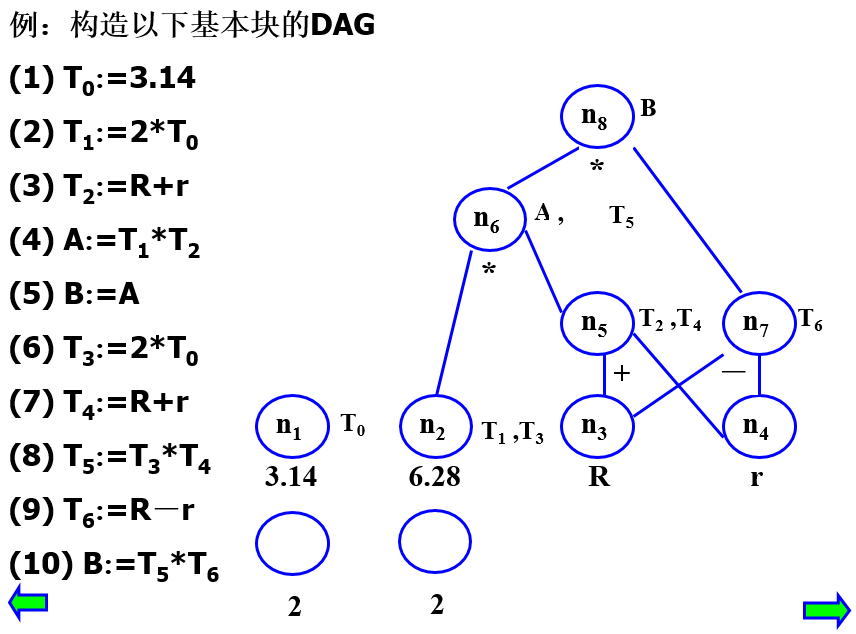
\includegraphics[scale = 0.3]{assets/CompilerConstructionPrinciples_723f0.png}
\end{figure}

\begin{figure}[H]
 \centering
 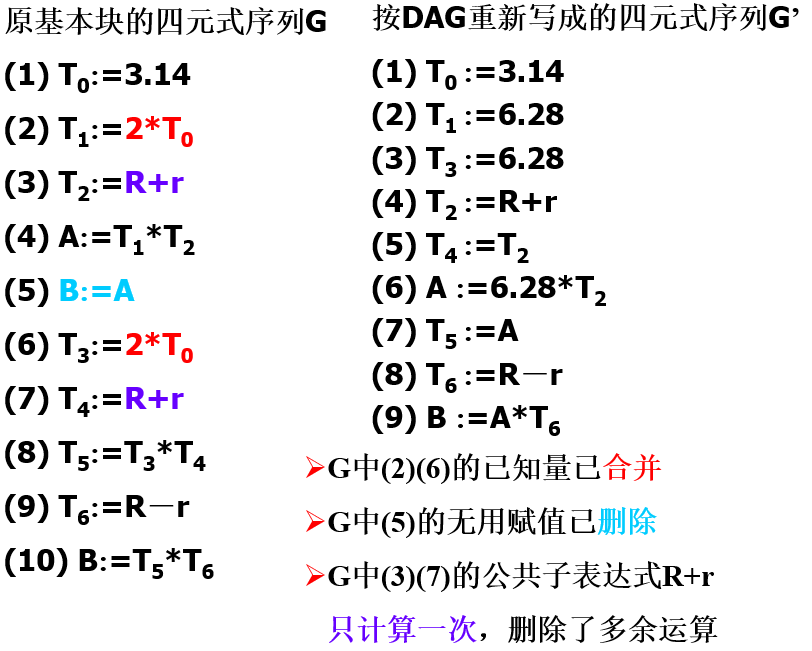
\includegraphics[scale = 0.3]{assets/CompilerConstructionPrinciples_e4017.png}
\end{figure}

\begin{figure}[H]
 \centering
 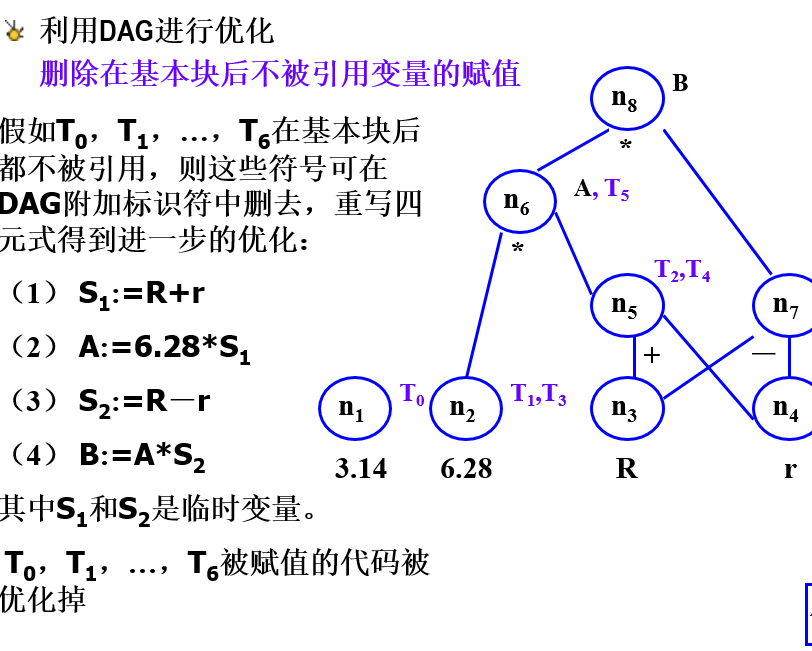
\includegraphics[scale = 0.3]{assets/CompilerConstructionPrinciples_e1d5a.png}
\end{figure}

\subsection{循环优化}
\begin{itemize}
 \item 代码外提\\
       把循环不变运算,即结果独立于循环执行次数的表达式,提到循环外面,使之只在循环外计算一次
 \item 强度削弱\\
       把程序中强度大的运算替换成强度小的运算\\
       比如把乘法运算换成加法运算
 \item 变换循环控制条件(删除归纳变量)
\end{itemize}

\end{document}
